\documentclass[10pt]{article}

% Pacotes extras necessários
\usepackage{amsmath}
\usepackage[lmargin=0.5in, rmargin=0.5in, tmargin=0.5in, bmargin=0.5in, includehead, includefoot]{geometry}
\usepackage{amsfonts}
\usepackage[utf8]{inputenc}
\usepackage[portuguese]{babel}
\usepackage{graphicx}
\usepackage{fancyhdr}
\usepackage{setspace}
\usepackage{listings}
\usepackage{url}
\usepackage{enumitem}
\usepackage{appendix} % For creating appendix sections
\usepackage{subcaption} % Use subcaption para legendas modernas

% More defined colors
\usepackage[dvipsnames]{xcolor}

% Define a custom style for the code listing
\lstdefinestyle{mystyle}{
    language=Matlab,
    inputencoding=latin1,
    extendedchars=true,
    backgroundcolor=\color{white},   % Choose the background color
    basicstyle=\ttfamily\footnotesize, % Set the font and size for the code
    numbers=left,                    % Line numbers on the left
    numberstyle=\tiny\color{gray},   % Line numbers style
    numbersep=5pt,                   % Distance of line numbers from the code
    tabsize=2,                       % Set tab size (default is 8 spaces)
    breaklines=true,                 % Automatically wrap long lines
    keywordstyle=\color{blue},       % Keywords in blue
    commentstyle=\color{green!60!black}, % Comments in green
    stringstyle=\color{orange},      % Strings in orange
    frame=single,                    % Draw a frame around the code
    keepspaces=true,                 % Preserve spaces in text
    showspaces=false,                % Don't show spaces in strings
    showstringspaces=false,          % Don't show spaces in strings
    showtabs=false,                  % Don't show tabs in strings
    % Add any other options you need
}

\lstset{style=mystyle} % Set the custom style
 
% Required package
\usepackage{tikz}
\usetikzlibrary{positioning}

\graphicspath{ {./images/} }

% Sets para outras partes
\setlength{\parindent}{1cm}
\setstretch{1.5}
\DeclareMathOperator{\sen}{sen}
\DeclareMathOperator{\sinc}{sinc}

%% Facilidades
%% -- Laplace
\newcommand{\Lap}[1]{\mathcal{L}\left\{#1\right\}}

%% -- Negrito em matemáticas
\newcommand{\bm}[1]{\boldsymbol{#1}}


% ------- Estilo do trabalho -------- %
\fancypagestyle{capa}{
    \fancyhf{}
    \renewcommand\headrulewidth{0pt}
}

\pagestyle{fancy}
\fancyhead{}
\fancyhead[L]{\thepage}
\fancyfoot{}
% ----------------------------------- %

% Dados do Grupo
\title{ Robótica e Automação - Trabalho Nº2}
\author{
    Leonardo Soares da Costa Tanaka - DRE: 121067652 \\
    Engenharia de Controle e Automação/UFRJ \\
    Rio de Janeiro, Brasil \\
    Dezembro de 2024
}
\date{}

\begin{document}
\maketitle
\thispagestyle{capa}

\section{Introdução}

Para a resolução do trabalho, foi o manipulador Kinova Gen3 Ultra lightweight (www.kinovarobotics.com) da Kinova
Inc.. A estrutura cinemática deste manipulador de 7 juntas pode ser vista na figura:

\begin{figure}[h]
    \centering
    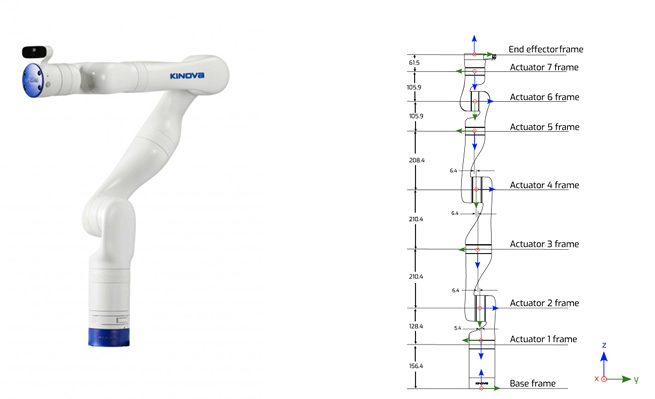
\includegraphics[scale=0.75]{kinova.png}
    \caption{Foto e Diagrama do manipulador Kinova}
\end{figure}

Além disso, os parâmetros de Denavit-Hartenberg do manipulador são apresentados na Tabela 1.
Foi considerado que a orientação do sistema de coordenadas 0 com relação à base é dado por
$R_{b0}=R_x(\pi)$ onde $R_x(\cdot)$ é uma rotação elementar ao redor do eixo x.

\begin{table}[h!]
    \centering
    \begin{tabular}{|c|c|c|c|c|c|}
    \hline
    \textbf{Junta} & $\alpha$ (rad) & $A$ (m) & $\theta$ (rad) & $D$ (m) & \textbf{Offset (rad)} \\ \hline
    1 & $\pi/2$ & 0 & $\theta_1$ & $-0.2848$ & $\pi$ \\ \hline
    2 & $\pi/2$ & 0 & $\theta_2$ & $-0.0118$ & $\pi$ \\ \hline
    3 & $\pi/2$ & 0 & $\theta_3$ & $-0.4208$ & $\pi$ \\ \hline
    4 & $\pi/2$ & 0 & $\theta_4$ & $-0.0128$ & $\pi$ \\ \hline
    5 & $\pi/2$ & 0 & $\theta_5$ & $-0.3143$ & $\pi$ \\ \hline
    6 & $\pi/2$ & 0 & $\theta_6$ & 0 & $\pi$ \\ \hline
    7 & $\pi$ & 0 & $\theta_7$ & 0 & $\pi$ \\ \hline
    \end{tabular}
    \caption{Parâmetros de Denavit-Hartenberg Standard do Kinova Gen3}
    \label{tab:dh_parameters}
\end{table}

Para a primeira parte do trabalho, foi considerado a posição inicial do manipulador é definida pelos ângulo das juntas:
$\theta = \begin{bmatrix} 0 & 15 & 180 & -130 & 0 & 55 & 90 \end{bmatrix}$ (graus). Porém, para a segunda parte do trabalho,
foi considerado a posição inicial do manipulador é definida pelos ângulos das juntas: $\theta_h = \begin{bmatrix} 90 & 15 & 180 & -130 & 0 & 55 & 0 \end{bmatrix}$ (graus).
Além disso, foi considerado que na tabela de Denavit-Hartenberg da primeira parte do trabalho tem o $d_7 = -0.3574 m$.

\section{Desenvolvimento}

\subsection{Controle Cinemático de Manipuladores}

Foi considerado o controle cinemático da posição do punho do manipulador
em que somente a Sinais de controle é controlada,
porque as 3 últimas juntas estão na mesma posição fazendo que as três últimas colunas do jacobiano sejam zero.
Além disso, a velocidade máxima das juntas foi definida como $\dot{\theta}_{max} = 1 \ rad/s$. Foram consideradas as seguintes trajétorias (com $\omega_n = \pi/2$):

\begin{enumerate}[label=(\alph*)]
    \item \( \mathbf{x}_d \) descreve uma circunferência de \( 0.1 \, \text{m} \) de raio no plano \( X-Z \), centrada no ponto $\mathbf{x}_0 = \begin{bmatrix} 0.4 & 0 & 0.4 \end{bmatrix}^T$,
    e percorrida com uma frequência \(\omega_n\).

    \item A circunferência do item anterior projetada no plano definido pela equação: $(x - 0.4) - y + (z - 0.4) = 0$.

    \item Considerando agora \(\omega_n = \frac{\pi}{8}\), temos:
    $\mathbf{x}_d(t) = \begin{bmatrix} 0.08 \big(\sin(\omega_n t) + \sin(4\omega_n t)\big) + 0.4 \\ 0 \\ 0.08 \big(\cos(\omega_n t) + \cos(4\omega_n t)\big) + 0.4 \end{bmatrix}.$
\end{enumerate}

Foi simulado o comportamento do sistema em malha fechada para as trajetórias especificadas utilizando os seguinte controladores:

\begin{enumerate}
    \item \( \mathbf{u} = \big(J(\boldsymbol{\theta})\big)^{\dagger} \mathbf{K} (\mathbf{x}_d - \mathbf{x}) \).
    
    \item \( \mathbf{u} = \big(J(\boldsymbol{\theta})\big)^{\dagger} \big[\dot{\mathbf{x}}_d + \mathbf{K} (\mathbf{x}_d - \mathbf{x})\big] \), onde $J^{\dagger} = J^\top \big(J J^\top\big)^{-1}$.
\end{enumerate}

Para implementar o segundo controlador, foi feita a derivação algébrica das três trajétórias consideradas no problema.
Portanto, não foi utilizado derivação numérica para definir o $\dot{x_d}$ no segundo controlador.
Além disso, foi sintonizado o ganho K com 6 configurações diferentes para obter o melhor desempenho possível atendendo a especificação de $|u_i| \leq 1 (i=1,2,3,4)$.
A seguir temos os gráficos utilizados para analisar as 6 configurações diferentes:

\newpage

\begin{figure}[h!]
    \centering
    \begin{subfigure}[b]{0.24\textwidth}
        \centering
        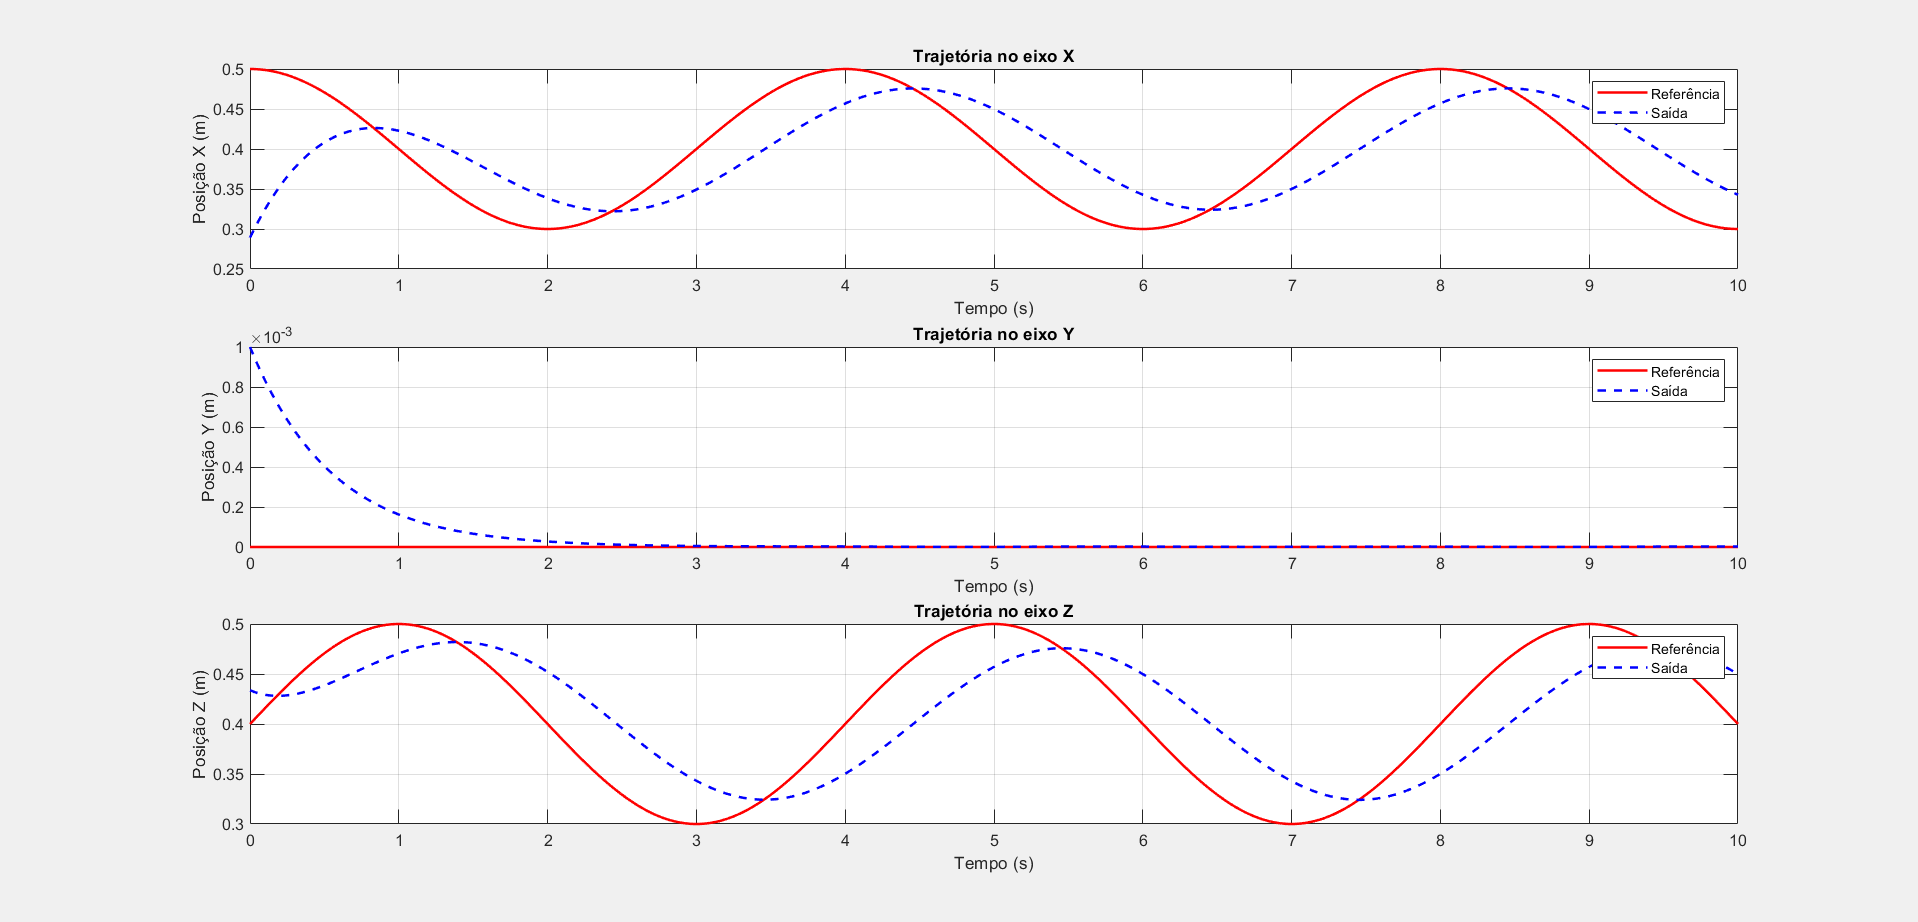
\includegraphics[width=\linewidth]{trajetorias_a1.png}
        \caption{Trajetórias nos eixos}
        \label{fig:trajetorias_a1}
    \end{subfigure}%
    \hfill
    \begin{subfigure}[b]{0.24\textwidth}
        \centering
        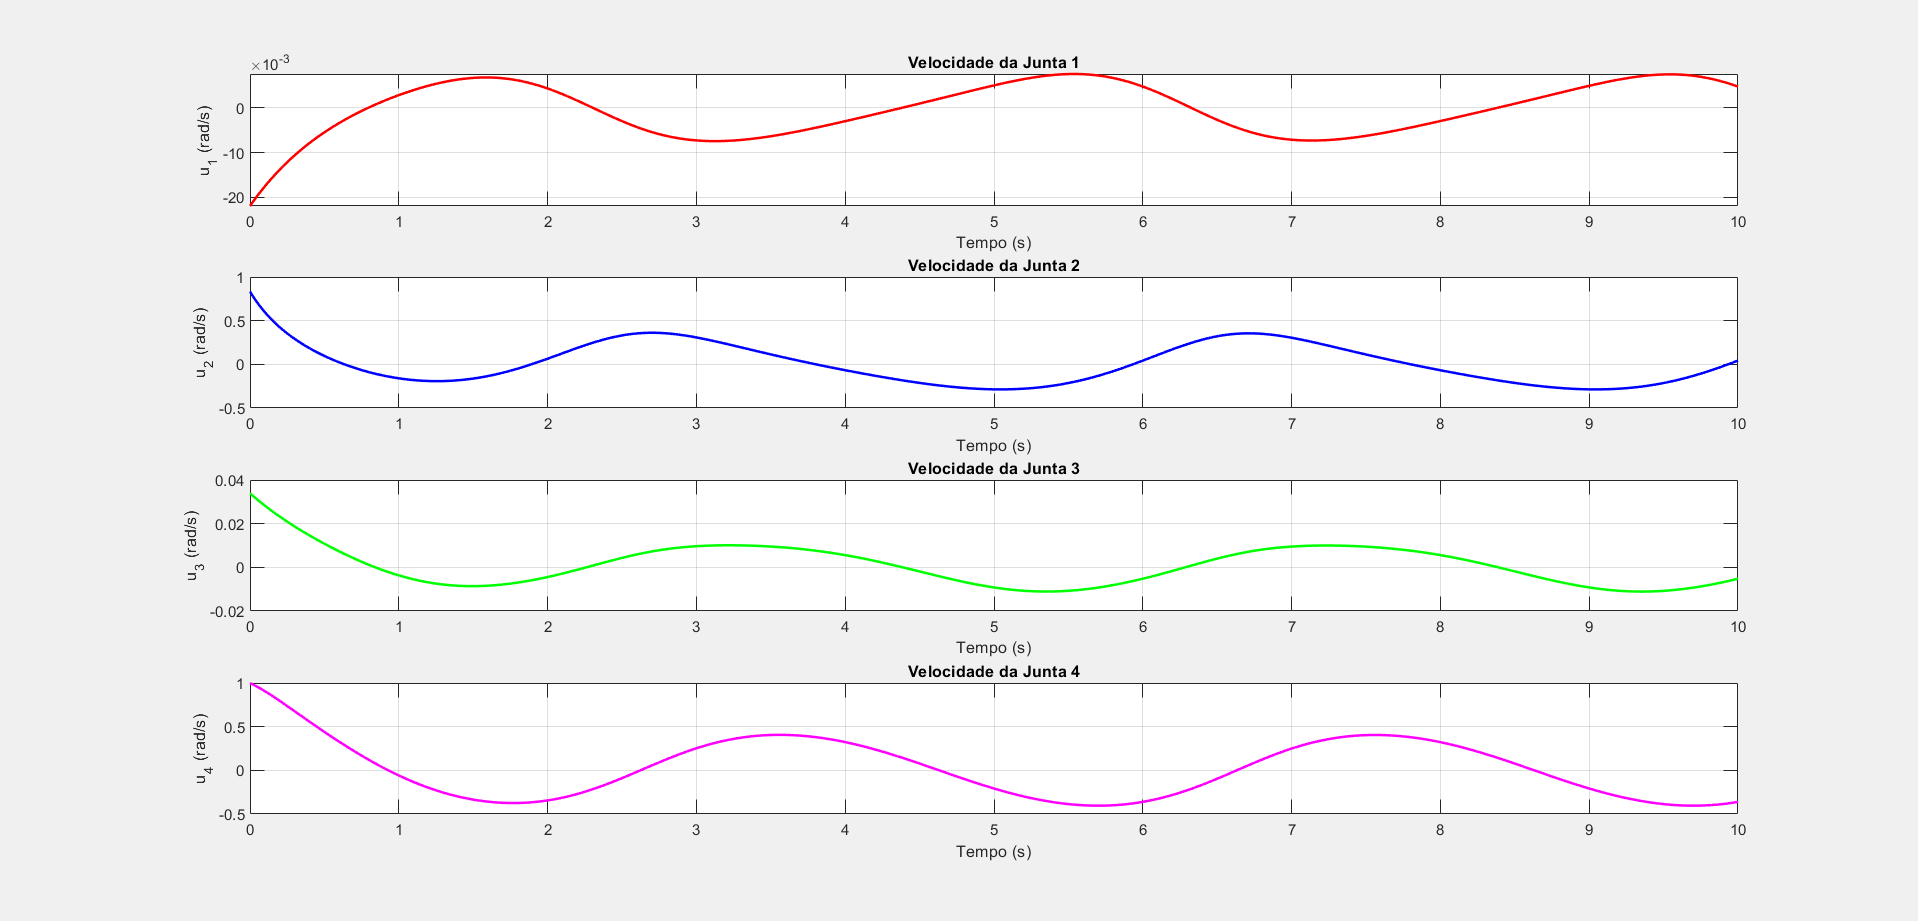
\includegraphics[width=\linewidth]{velocidades_a1.png}
        \caption{Sinais de controle}
        \label{fig:velocidades_a1}
    \end{subfigure}%
    \hfill
    \begin{subfigure}[b]{0.24\textwidth}
        \centering
        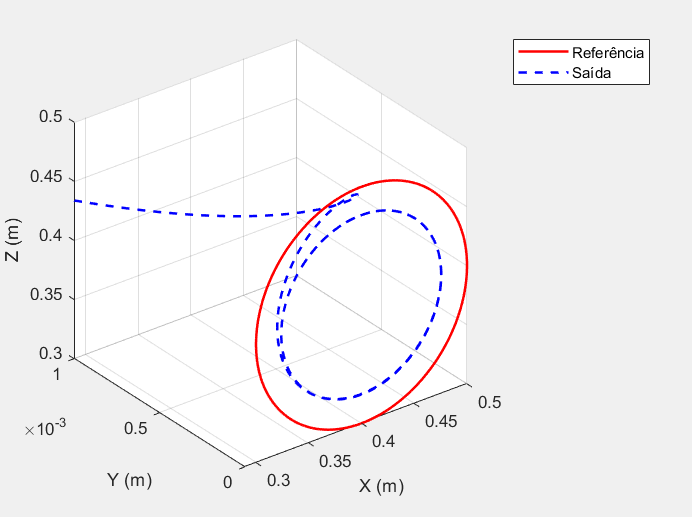
\includegraphics[width=\linewidth]{grafico3d_a1.png}
        \caption{Trajetória no espaço}
        \label{fig:grafico3d_a1}
    \end{subfigure}%
    \hfill
    \begin{subfigure}[b]{0.24\textwidth}
        \centering
        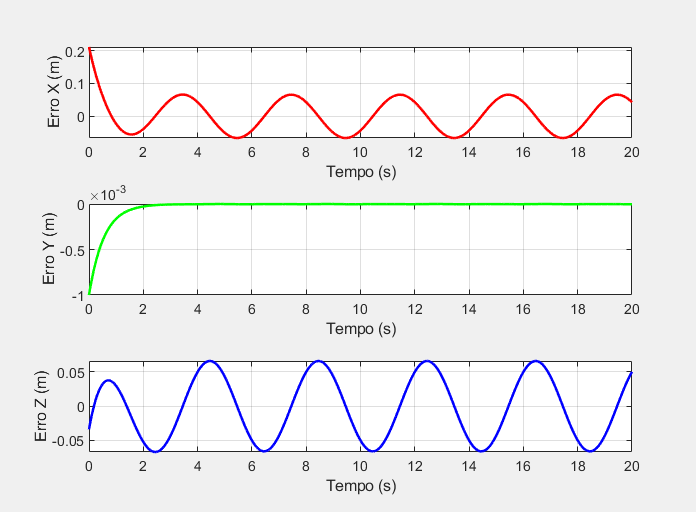
\includegraphics[width=\linewidth]{erro_a1.png}
        \caption{Erro nas posições}
        \label{fig:erro_a1}
    \end{subfigure}
    \caption{Gráficos da Trajetória (a) com Controlador 1 (K = 1.81)}
    \label{fig:a1}
\end{figure}

\begin{figure}[h!]
    \centering
    \begin{subfigure}[b]{0.24\textwidth}
        \centering
        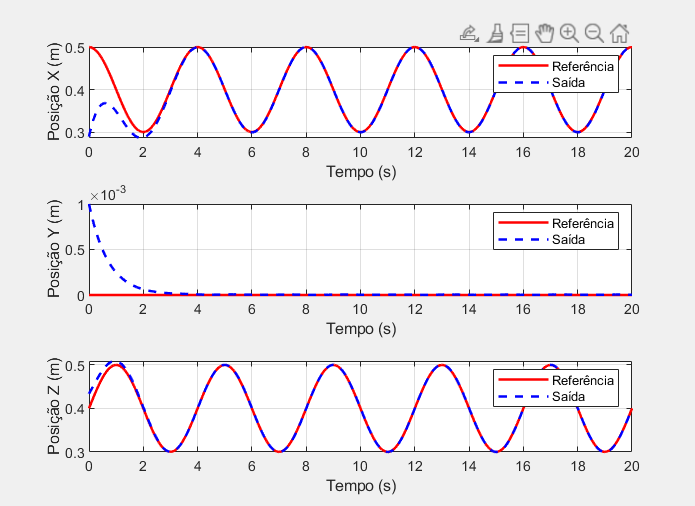
\includegraphics[width=\linewidth]{trajetorias_a2.png}
        \caption{Trajetórias nos eixos}
        \label{fig:trajetorias_a2}
    \end{subfigure}%
    \hfill
    \begin{subfigure}[b]{0.24\textwidth}
        \centering
        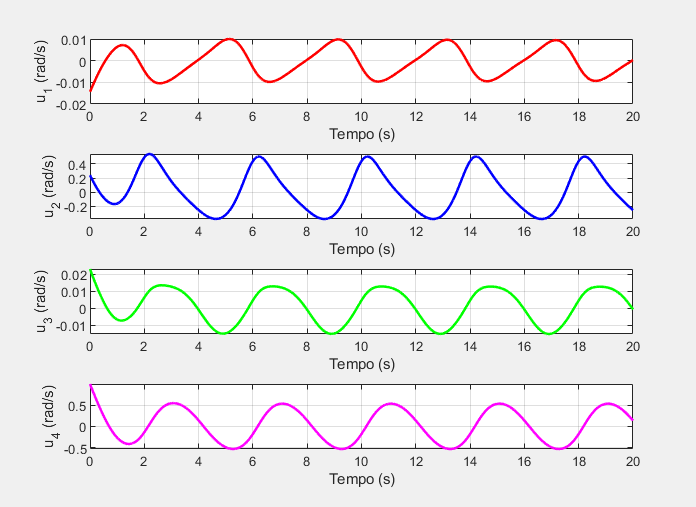
\includegraphics[width=\linewidth]{velocidades_a2.png}
        \caption{Sinais de controle}
        \label{fig:velocidades_a2}
    \end{subfigure}%
    \hfill
    \begin{subfigure}[b]{0.24\textwidth}
        \centering
        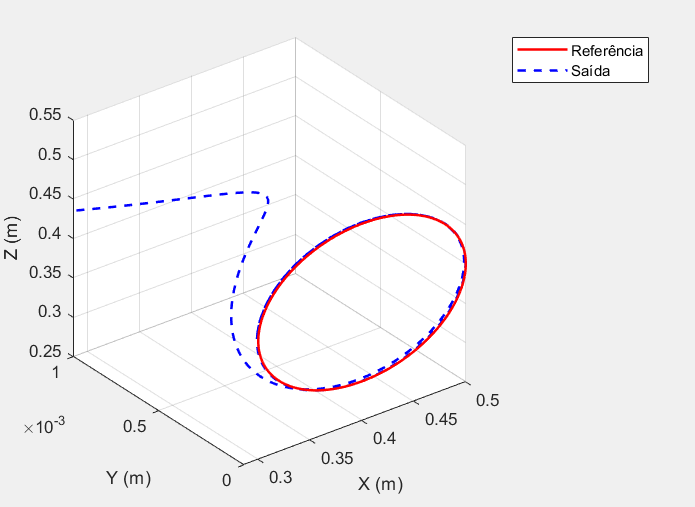
\includegraphics[width=\linewidth]{grafico3d_a2.png}
        \caption{Trajetória no espaço}
        \label{fig:grafico3d_a2}
    \end{subfigure}%
    \hfill
    \begin{subfigure}[b]{0.24\textwidth}
        \centering
        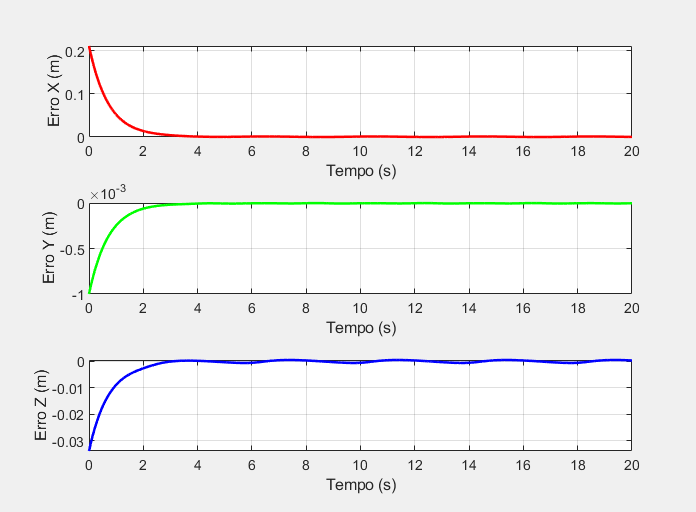
\includegraphics[width=\linewidth]{erro_a2.png}
        \caption{Erro nas posições}
        \label{fig:erro_a2}
    \end{subfigure}
    \caption{Gráficos da Trajetória (a) com Controlador 2 (K = 1.39)}
    \label{fig:a2}
\end{figure}

\begin{figure}[h!]
    \centering
    \begin{subfigure}[b]{0.24\textwidth}
        \centering
        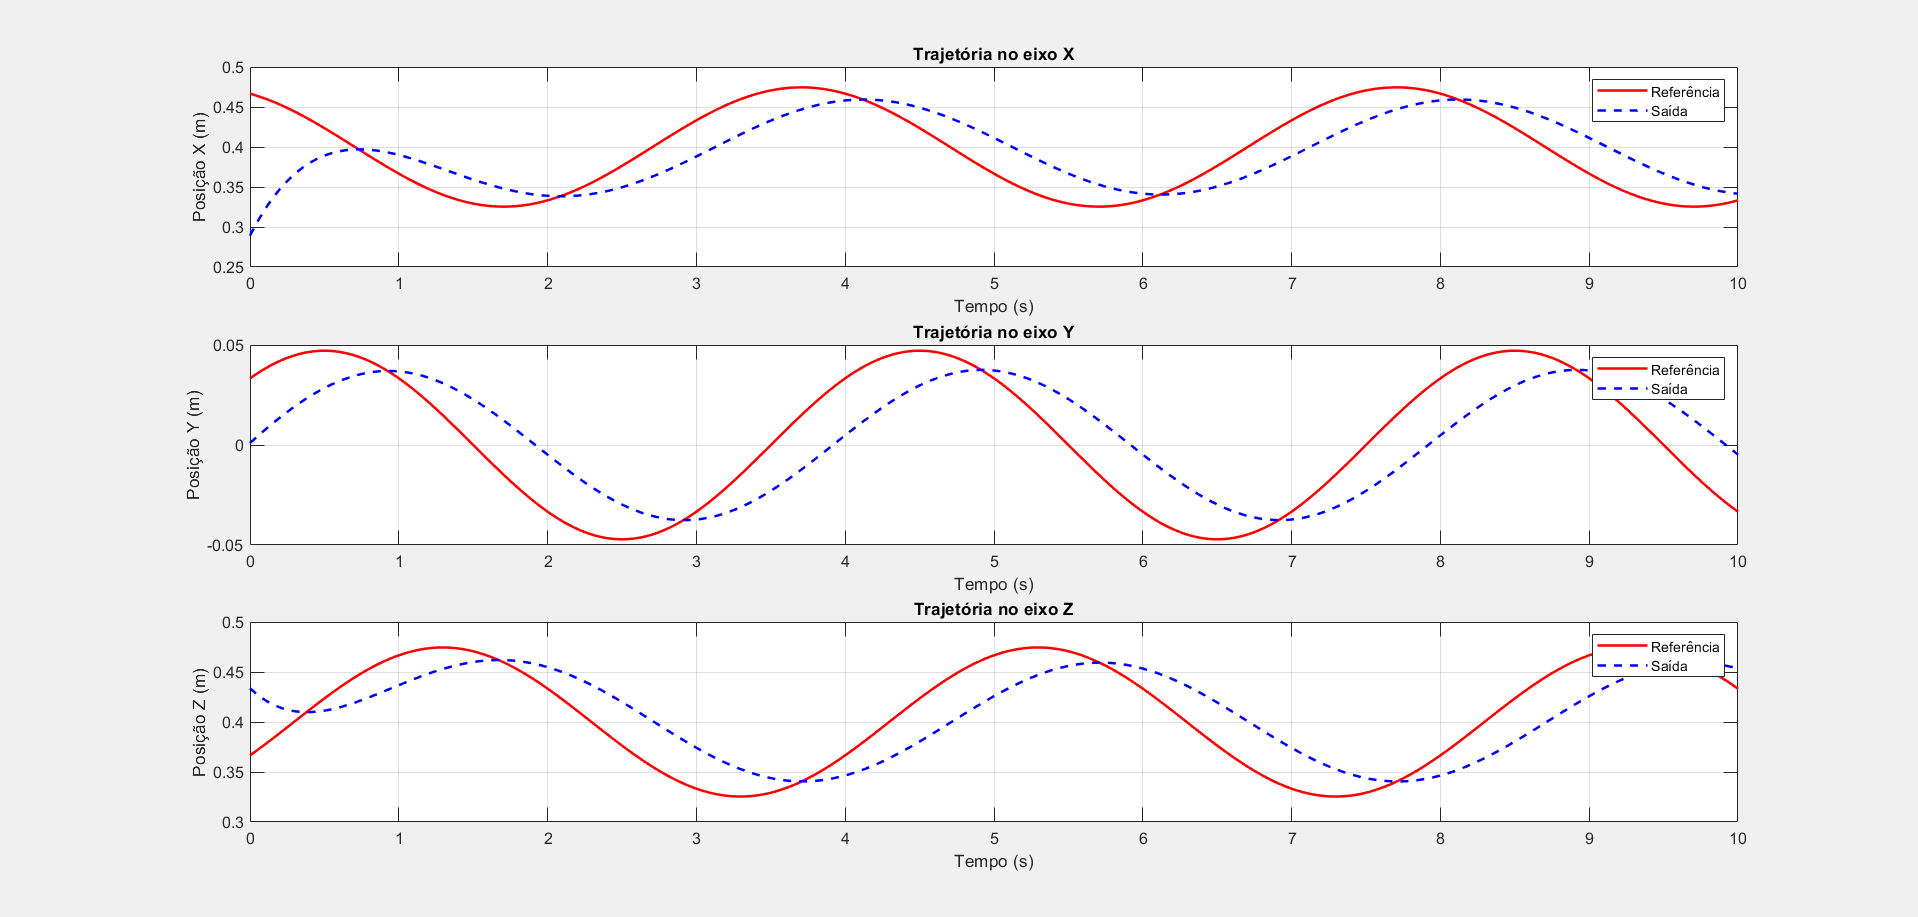
\includegraphics[width=\linewidth]{trajetorias_b1.png}
        \caption{Trajetórias nos eixos}
        \label{fig:trajetorias_b1}
    \end{subfigure}%
    \hfill
    \begin{subfigure}[b]{0.24\textwidth}
        \centering
        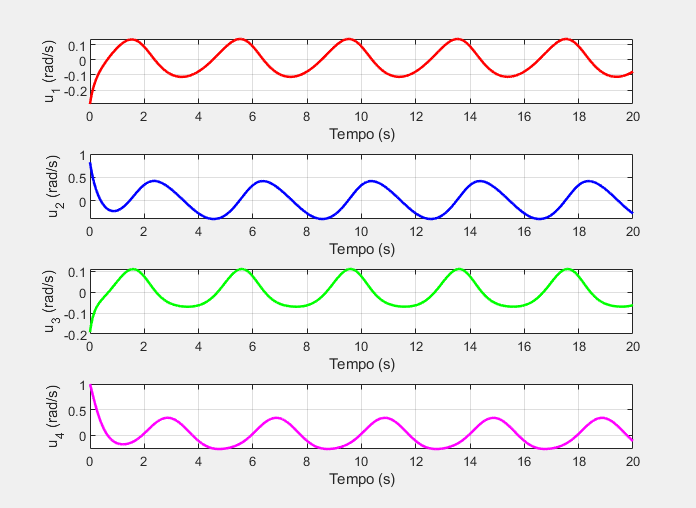
\includegraphics[width=\linewidth]{velocidades_b1.png}
        \caption{Sinais de controle}
        \label{fig:velocidades_b1}
    \end{subfigure}%
    \hfill
    \begin{subfigure}[b]{0.24\textwidth}
        \centering
        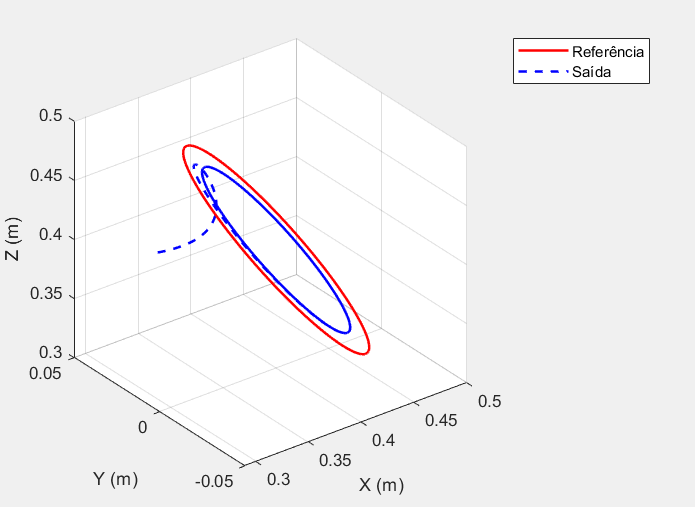
\includegraphics[width=\linewidth]{grafico3d_b1.png}
        \caption{Trajetória no espaço}
        \label{fig:grafico3d_b1}
    \end{subfigure}%
    \hfill
    \begin{subfigure}[b]{0.24\textwidth}
        \centering
        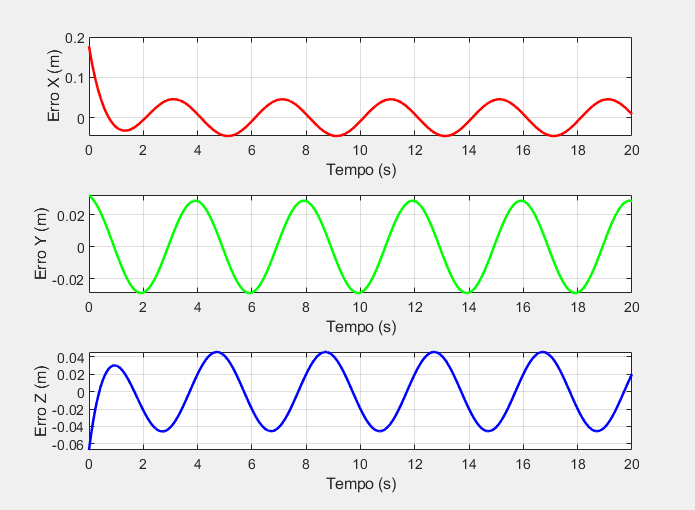
\includegraphics[width=\linewidth]{erro_b1.png}
        \caption{Erro nas posições}
        \label{fig:erro_b1}
    \end{subfigure}
    \caption{Gráficos da Trajetória (b) com Controlador 1 (K = 2.05)}
    \label{fig:b1}
\end{figure}

\begin{figure}[h!]
    \centering
    \begin{subfigure}[b]{0.24\textwidth}
        \centering
        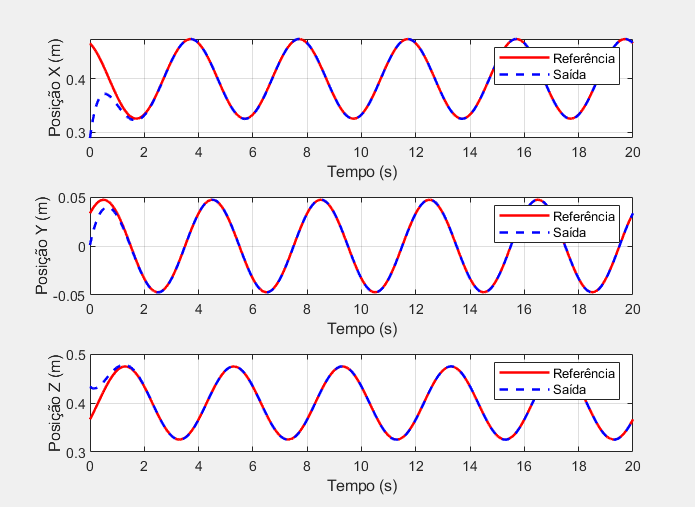
\includegraphics[width=\linewidth]{trajetorias_b2.png}
        \caption{Trajetórias nos eixos}
        \label{fig:trajetorias_b2}
    \end{subfigure}%
    \hfill
    \begin{subfigure}[b]{0.24\textwidth}
        \centering
        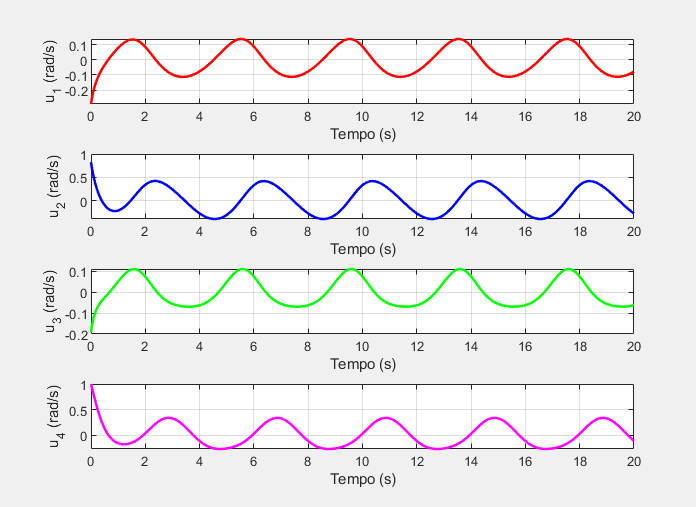
\includegraphics[width=\linewidth]{velocidades_b2.png}
        \caption{Sinais de controle}
        \label{fig:velocidades_b2}
    \end{subfigure}%
    \hfill
    \begin{subfigure}[b]{0.24\textwidth}
        \centering
        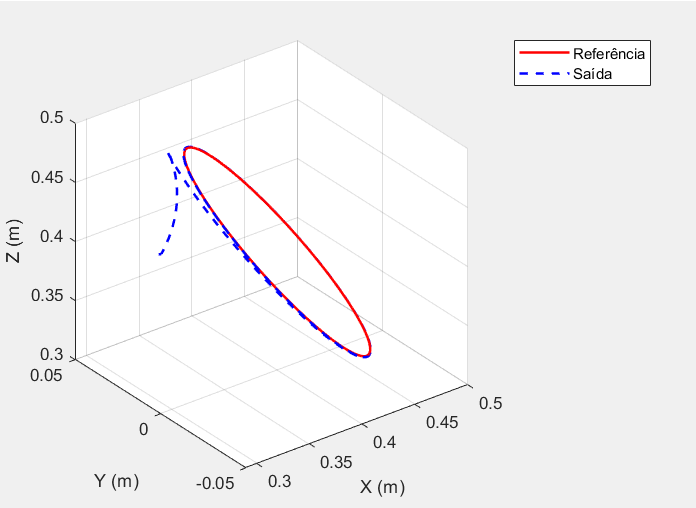
\includegraphics[width=\linewidth]{grafico3d_b2.png}
        \caption{Trajetória no espaço}
        \label{fig:grafico3d_b2}
    \end{subfigure}%
    \hfill
    \begin{subfigure}[b]{0.24\textwidth}
        \centering
        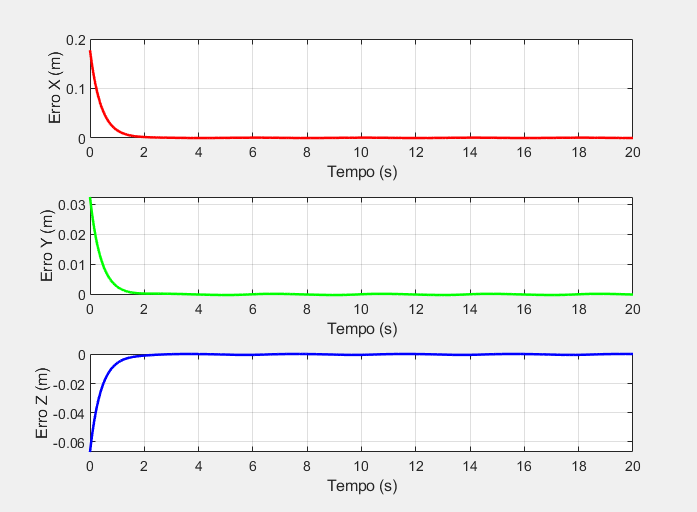
\includegraphics[width=\linewidth]{erro_b2.png}
        \caption{Erro nas posições}
        \label{fig:erro_b2}
    \end{subfigure}
    \caption{Gráficos da Trajetória (b) com Controlador 2 (K = 2.42)}
    \label{fig:b2}
\end{figure}

\newpage

\begin{figure}[h!]
    \centering
    \begin{subfigure}[b]{0.24\textwidth}
        \centering
        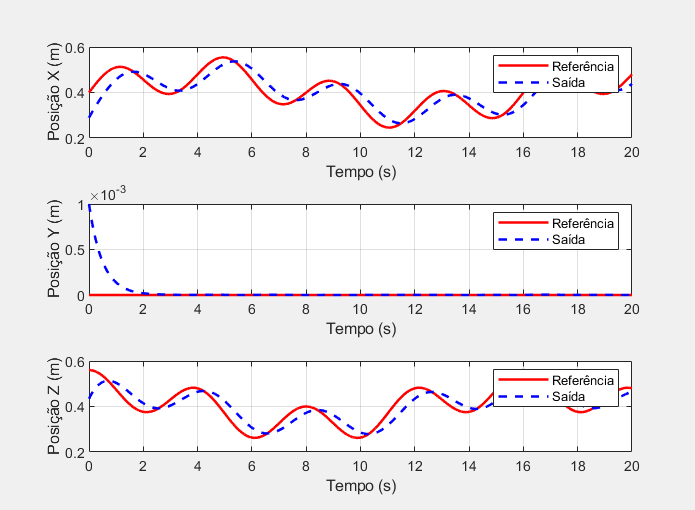
\includegraphics[width=\linewidth]{trajetorias_c1.png}
        \caption{Trajetórias nos eixos}
        \label{fig:trajetorias_c1}
    \end{subfigure}%
    \hfill
    \begin{subfigure}[b]{0.24\textwidth}
        \centering
        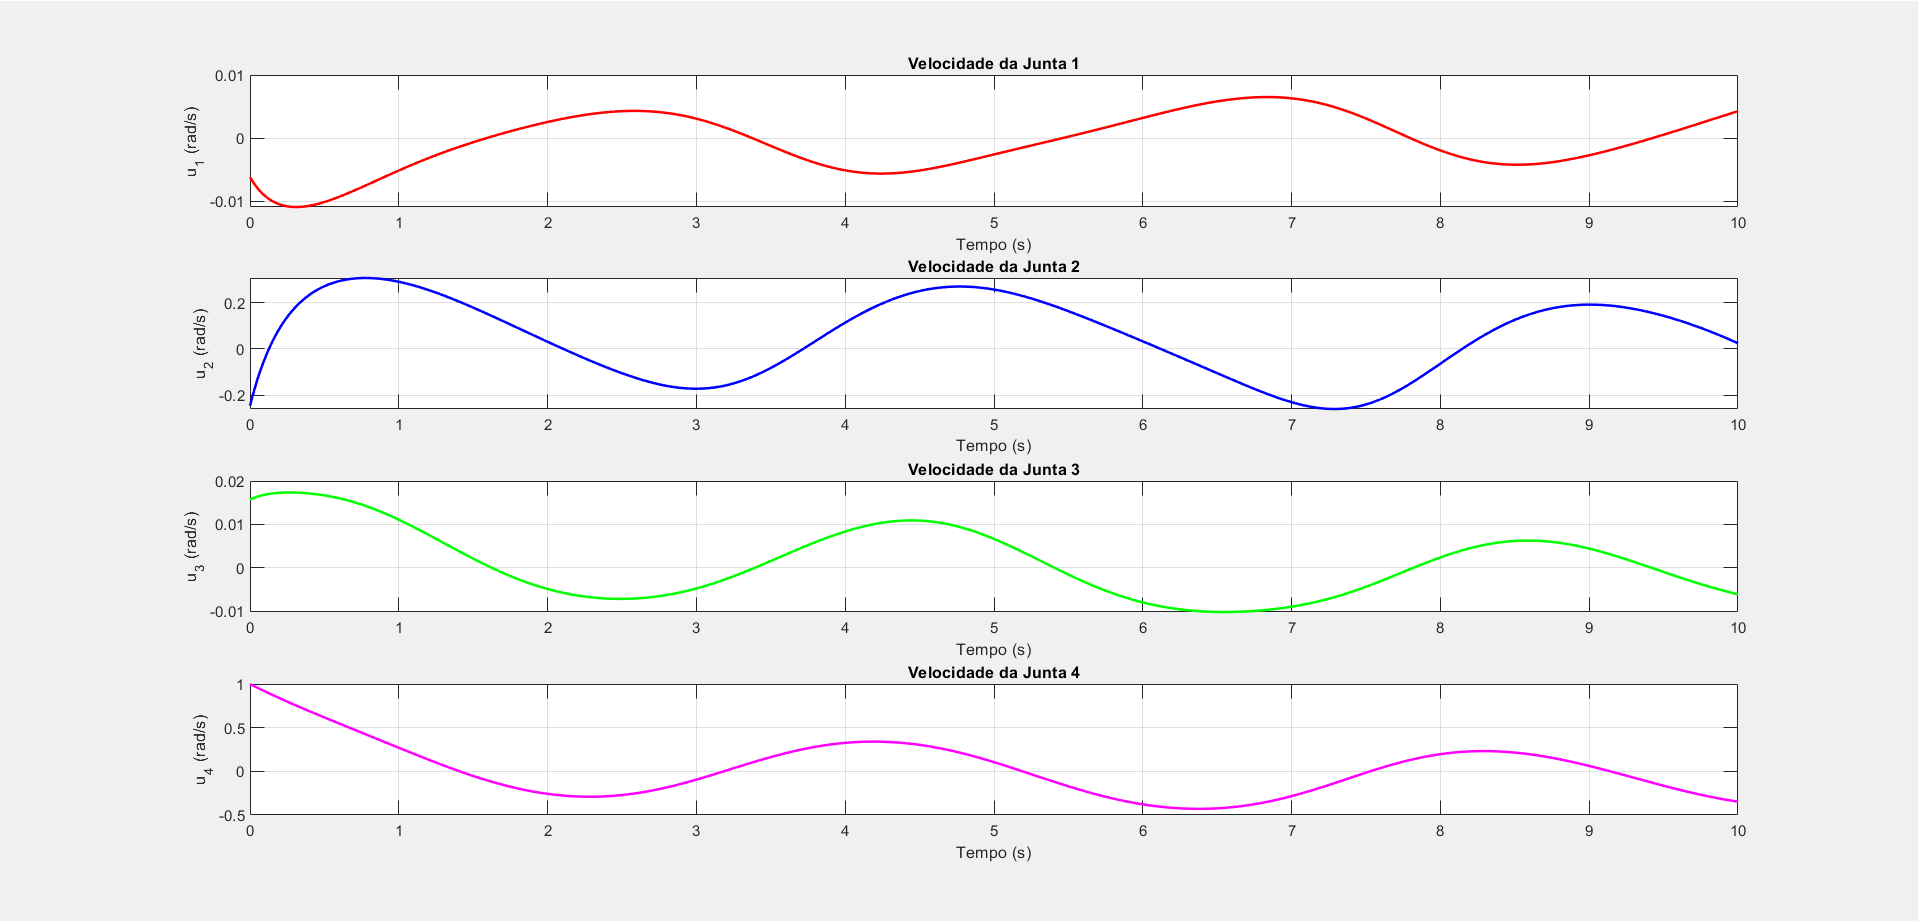
\includegraphics[width=\linewidth]{velocidades_c1.png}
        \caption{Sinais de controle}
        \label{fig:velocidades_c1}
    \end{subfigure}%
    \hfill
    \begin{subfigure}[b]{0.24\textwidth}
        \centering
        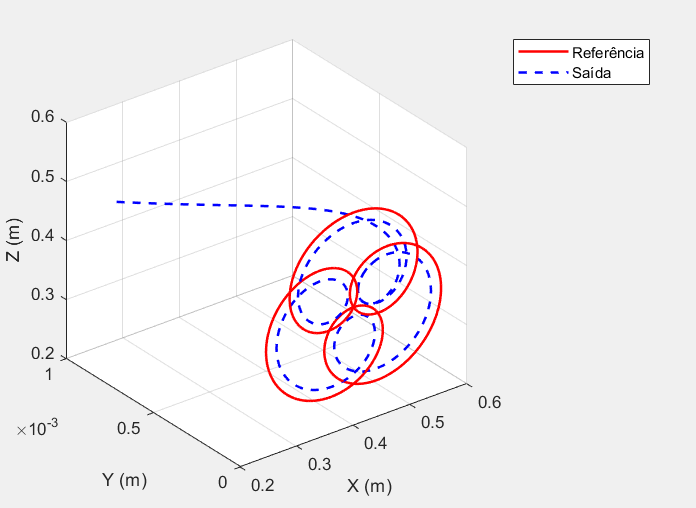
\includegraphics[width=\linewidth]{grafico3d_c1.png}
        \caption{Trajetória no espaço}
        \label{fig:grafico3d_c1}
    \end{subfigure}%
    \hfill
    \begin{subfigure}[b]{0.24\textwidth}
        \centering
        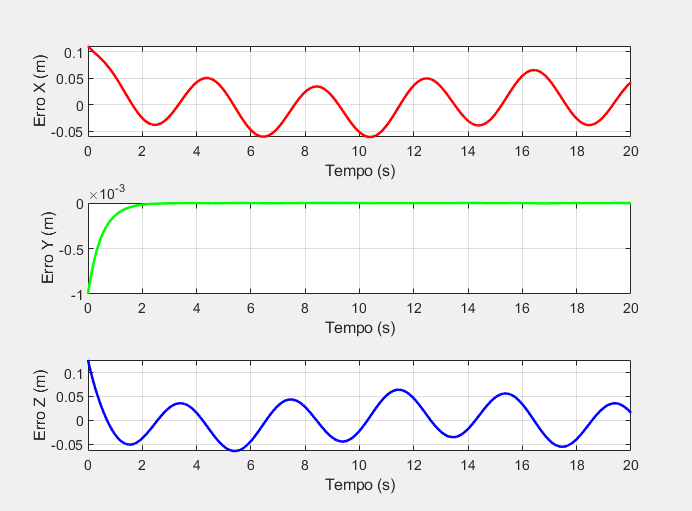
\includegraphics[width=\linewidth]{erro_c1.png}
        \caption{Erro nas posições}
        \label{fig:erro_c1}
    \end{subfigure}
    \caption{Gráficos da Trajetória (c) com Controlador 1 (K = 1.99)}
    \label{fig:c1}
\end{figure}

\begin{figure}[h!]
    \centering
    \begin{subfigure}[b]{0.24\textwidth}
        \centering
        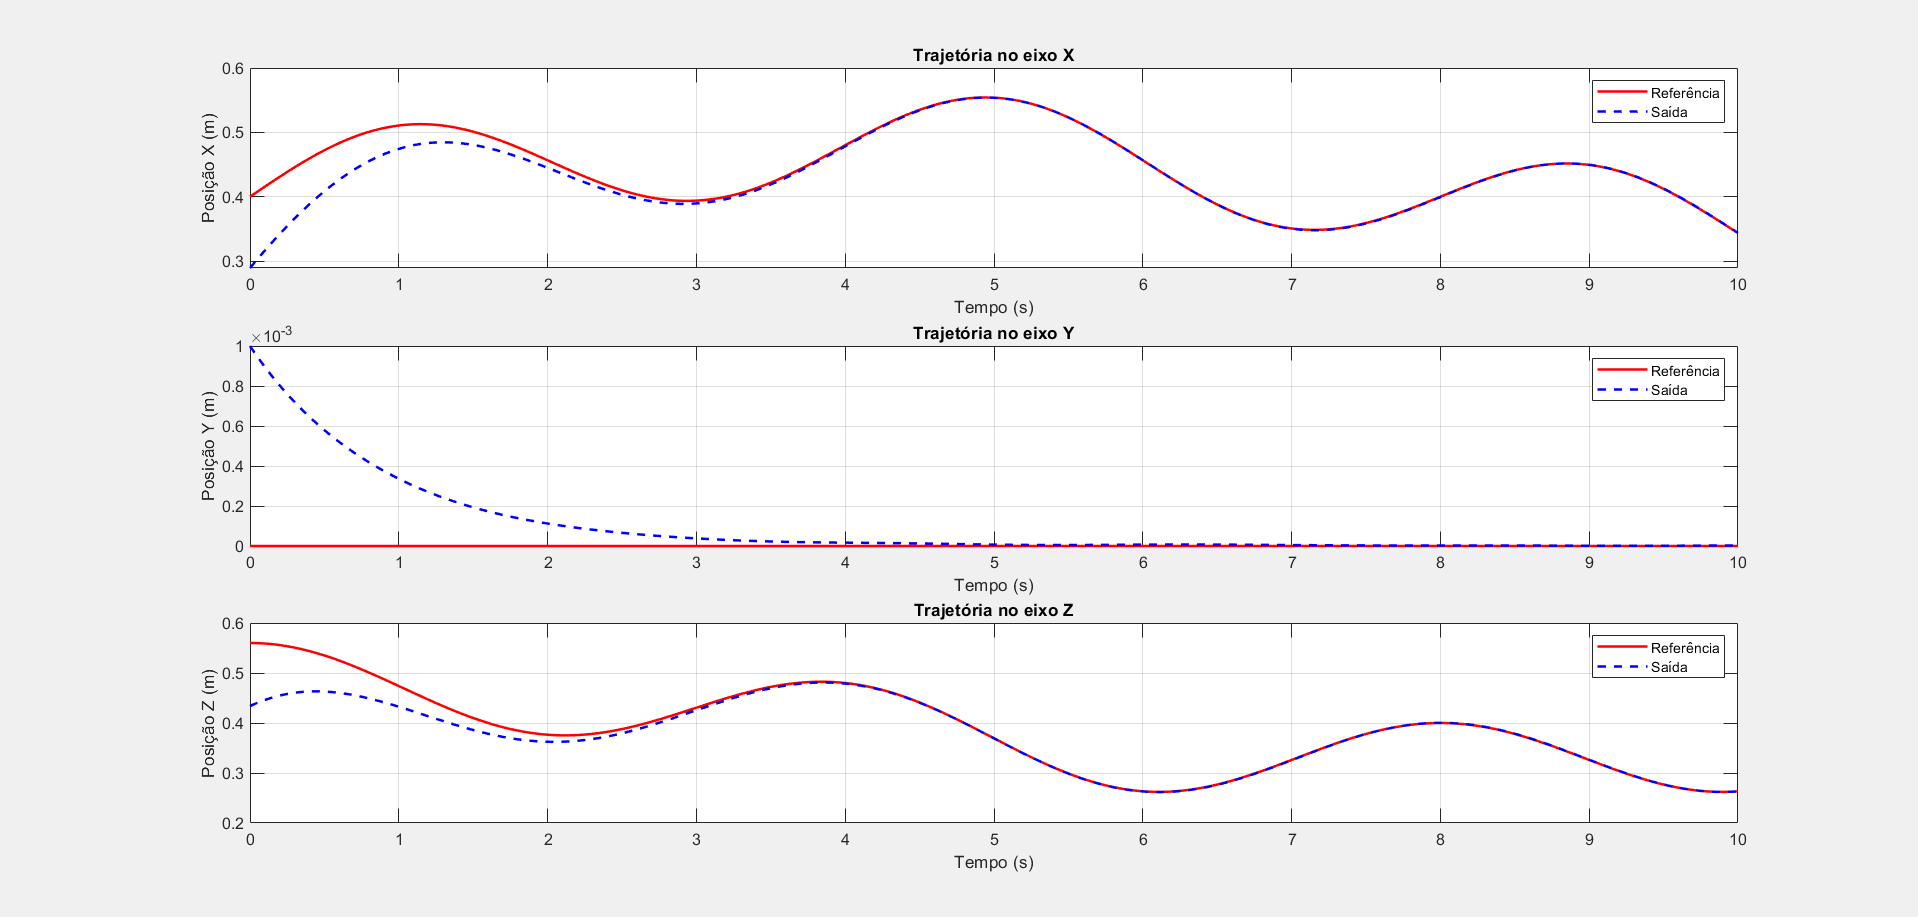
\includegraphics[width=\linewidth]{trajetorias_c2.png}
        \caption{Trajetórias nos eixos}
        \label{fig:trajetorias_c2}
    \end{subfigure}%
    \hfill
    \begin{subfigure}[b]{0.24\textwidth}
        \centering
        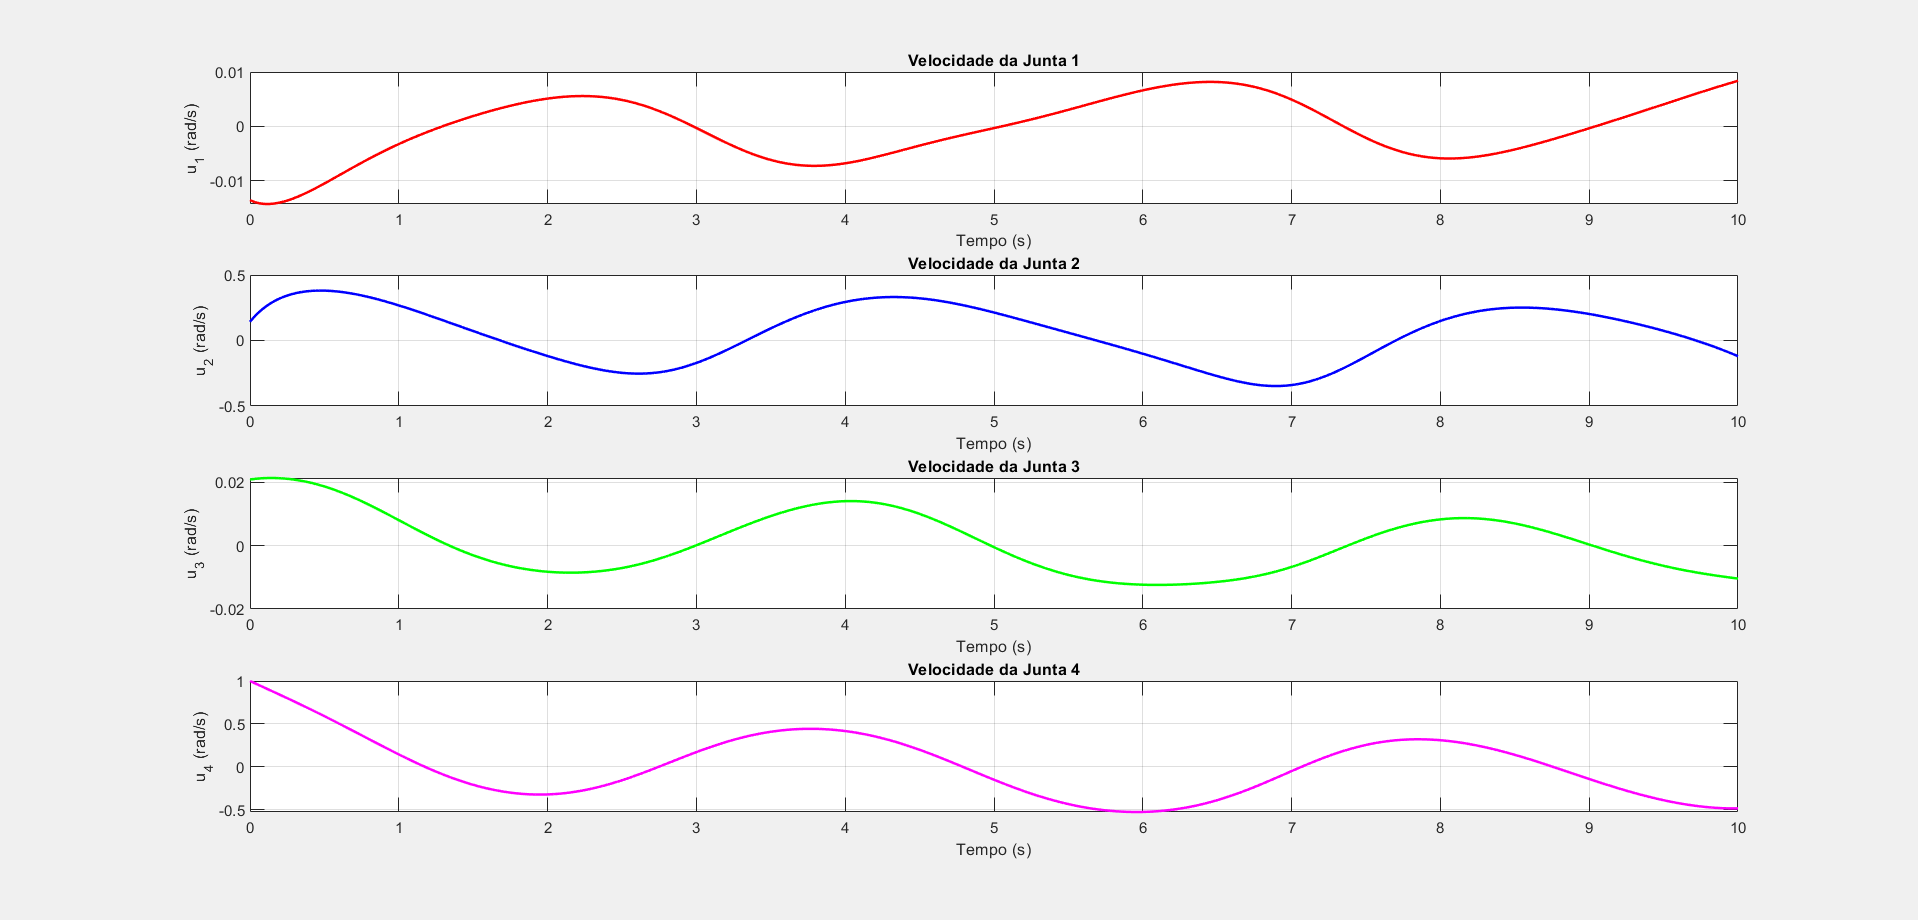
\includegraphics[width=\linewidth]{velocidades_c2.png}
        \caption{Sinais de controle}
        \label{fig:velocidades_c2}
    \end{subfigure}%
    \hfill
    \begin{subfigure}[b]{0.24\textwidth}
        \centering
        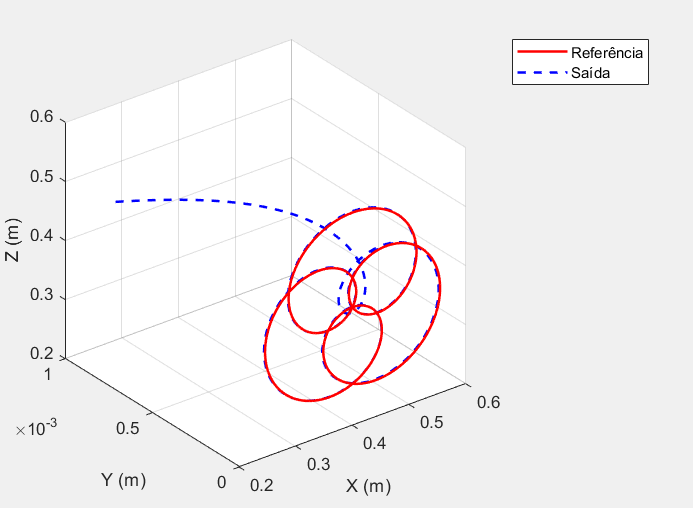
\includegraphics[width=\linewidth]{grafico3d_c2.png}
        \caption{Trajetória no espaço}
        \label{fig:grafico3d_c2}
    \end{subfigure}%
    \hfill
    \begin{subfigure}[b]{0.24\textwidth}
        \centering
        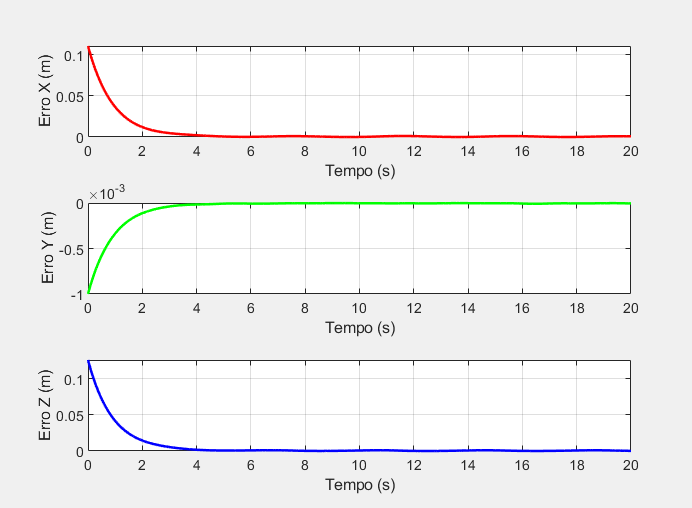
\includegraphics[width=\linewidth]{erro_c2.png}
        \caption{Erro nas posições}
        \label{fig:erro_c2}
    \end{subfigure}
    \caption{Gráficos da Trajetória (c) com Controlador 2 (K = 2.17)}
    \label{fig:c2}
\end{figure}

Após analisar os dados obtidos das 6 configurações diferentes, é possível concluir sobre a estabilidade e desempenho de cada um dos controladores.
Portanto, os controladores podem assegurar a estabilidade, se $J(\theta)$ tenha posto completo, garantindo a existência do pseudo-inverso $(J^{\dagger})$.
Além disso, o controlador 1 não consegue ter a convergência ao ser respeitado as especificações do problema.
Assim, a saída acaba tendo uma diferença de fase em relação a trajetória de referência e um desvio considerável para as três trajetórias especificadas,
o que demonstra um desempenho ruim para seguimento de trajetórias.
Entretanto, o controlador 2 consegue ter a convergência ao ser respeitado as especificações do problema.
Ademais, o erro entre a saída e a trajetória de referência acaba tendendo a zero de uma forma bem rápida,
tendo um desempenho bom para seguimento de trajetórias. 
Isso acontece, porque o controlador 2 possui uma feedforward $(\dot{x_d})$ compensando o movimento desejado.

\subsection{Controle Cinemático de Manipuladores por Servo Visão}

Para o controle cinemático da posição do efetuador utilizando servo-visão,
foi considerado somente os comandos de velocidade das juntas {1,2,4,6}.
Assim, considerando as juntas {3,5,7} fixas, i.e. $\dot{\theta}_3 = \dot{\theta}_5 = \dot{\theta}_7 = 0$.
Além disso, foi utilizada uma câmera monocular com eixo ótico (x) é perpendicular ao plano de trabalho (x-y) do manipulador,
a distância focal é $f=4mm$, posição a uma distância de $z_0=0.4338m$ do plano de trabalho do manipulador e
o fator de escala é $\alpha = 200000$ pixels/m nas duas direções.
Ademais, foi definido a origem do plano da imagem $O_c = \begin{bmatrix} 320 & 240 \end{bmatrix}^T$ e 
a posição da cãmera com relação à base do manipulador é $P_{bc} = \begin{bmatrix} 0 & -0.603 & 0 \end{bmatrix}^T$
com orientação $\phi = 0$, i.e. $R_{bc} = I$. Foi considerada seguinte trajetória em coordenada da tela (com $\omega_n = 0.5$):

\begin{equation}
    x_{cd} = \begin{bmatrix}
        360 - 30 \cos(\omega_n t) - 30 \cos(1.5 \omega_n t) - 10 \cos(2 \omega_n t) \\
        150 - 20 \cos(\omega_n t + 1.6) - 20 \cos(1.5 \omega_n t + 1.6) - 10 \cos(2 \omega_n t + 1.6)
    \end{bmatrix}
\end{equation}

Também, foi feito a derivação algébrica da trajetória para utilizar o controle 2 da subseção anterior:

\begin{equation}
    \dot{x}_{cd} = \begin{bmatrix}
        30 \sin(\omega_n t) \omega_n + 45 \sin(1.5 \omega_n t) 1.5 \omega_n + 20 \sin(2 \omega_n t) 2 \omega_n \\
        20 \sin(\omega_n t + 1.6) \omega_n + 30 \sin(1.5 \omega_n t + 1.6) 1.5 \omega_n + 20 \sin(2 \omega_n t + 1.6) 2 \omega_n
    \end{bmatrix}
\end{equation}

A partir das informações acima foi feita um estudo em relação ao controle por servo-visão.
Assim, temos a seguir certos conceitos que foram necessários para fazer o código de solução do problema no Matlab.
A transformação câmera/espaço de trabalho é dada por:

\begin{equation}
\text{x}_c = K_p \cdot \text{x} + \text{x}_{c0}
\end{equation}
onde
\begin{equation}
K_p = \frac{f}{z_0} \begin{bmatrix}
\alpha_1 & 0 \\
0 & \alpha_2
\end{bmatrix}
\end{equation}
e
\begin{equation}
\text{x}_{c0} = \frac{f}{z_0} \begin{bmatrix}
\alpha_1 & 0 \\
0 & \alpha_2
\end{bmatrix}
\begin{bmatrix}
    \cos(\phi) & \sin(\phi) \\
    \sin(\phi) & -\cos(\phi)
\end{bmatrix} P_{bc}
+ \begin{bmatrix}
    O_1 \\
    O_2
\end{bmatrix}
\end{equation}
em que
\begin{itemize}
    \item $\text{x}_c$: posição do efetuador no sistema de coordenadas da imagem.
    \item $\text{x}_c^0$: offset da posição do frame da câmera com respeito ao do robô.
    \item $K_p$: orientação e escalamento da câmera com respeito ao robô.
    \item $\phi$: ângulo de orientação da câmera com respeito ao frame do robô.
    \item $f$: distância focal da câmera.
    \item $z_0$: profundidade do plano da imagem ao plano de trabalho do robô.
    \item $\alpha_i > 0$: fatores de escala (pixels/m).
\end{itemize}

No sistema de coordenadas da câmera, a cinemática diferencial é dada por:

\begin{equation}
\dot{x}_c = K_p \dot{x}, \quad \mathbf{x}^T = [x_1, x_2]
\end{equation}
em que \( \mathbf{x}_{cd} \in \mathbb{R}^2 \) é a trajetória desejada do efetuador no plano da câmera. Uma lei de controle cartesiano pode ser projetada para que \( \mathbf{x}_c \to \mathbf{x}_{cd} \), ou seja, \( e_{cd} \to 0 \).
A equação dinâmica de \( e_{cd} \) é dada por:

\begin{equation}
\dot{e}_{cd} = \dot{x}_{cd} - \dot{x}_c = \dot{x}_{cd} - K_p J(\theta) u
\end{equation}

Com uma lei de controle dada por:

\begin{equation}
u = (K_p J(\theta))^{-1} \left[ \dot{x}_{cd} + K ( \mathbf{x}_{cd} - \mathbf{x}_c ) \right]
\end{equation}

O sistema em malha fechada é dado por:

\begin{equation}
\dot{e}_{cd} + K e_{cd} = 0 \quad \text{para} \quad K > 0
\end{equation}

O sistema é exponencialmente estável, com a solução:

\begin{equation}
e_{cd}(t) = e^{-Kt} e_{cd}(0)
\end{equation}

Primeiramente, foi simulado o controle por servo-visão do efetuador com $K = 1$ para avaliar a estabilidade, tendo os seguintes resultados:

\begin{figure}[h!]
    \centering
    \begin{subfigure}[b]{0.3\textwidth}
        \centering
        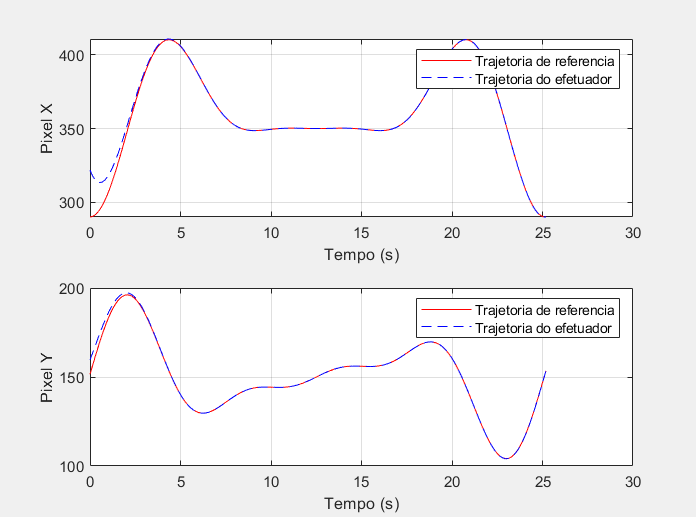
\includegraphics[width=\linewidth]{parte2_trajetorias_1.png}
        \caption{Trajetórias nos eixos X e Y}
        \label{fig:parte2_trajetorias_1}
    \end{subfigure}%
    \hfill
    \begin{subfigure}[b]{0.3\textwidth}
        \centering
        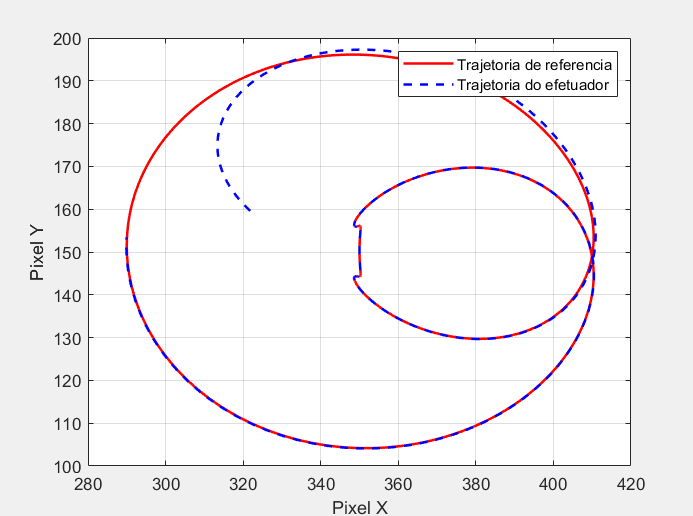
\includegraphics[width=\linewidth]{parte2_trajetoriaxy_1.png}
        \caption{Trajetória no plano X-Y}
        \label{fig:parte2_trajetoriaxy_1}
    \end{subfigure}%
    \hfill
    \begin{subfigure}[b]{0.3\textwidth}
        \centering
        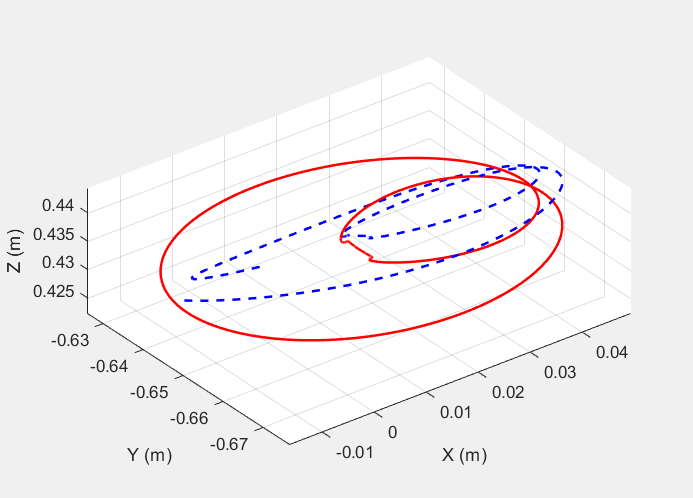
\includegraphics[width=\linewidth]{parte2_trajetoriaxyz_1.png}
        \caption{Trajetória no espaço XYZ}
        \label{fig:parte2_trajetoriaxyz_1}
    \end{subfigure}
    \begin{subfigure}[b]{0.3\textwidth}
        \centering
        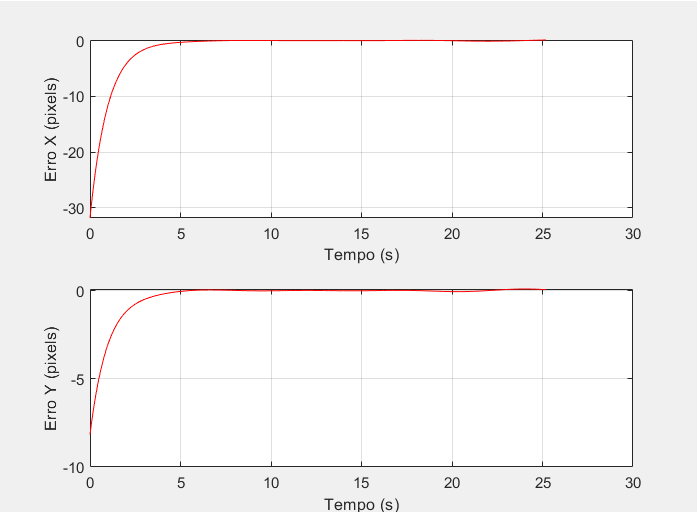
\includegraphics[width=\linewidth]{parte2_erro_1.png}
        \caption{Erro de posição nos eixos X e Y}
        \label{fig:parte2_erro_1}
    \end{subfigure}
    \hspace{1cm}
    \begin{subfigure}[b]{0.3\textwidth}
        \centering
        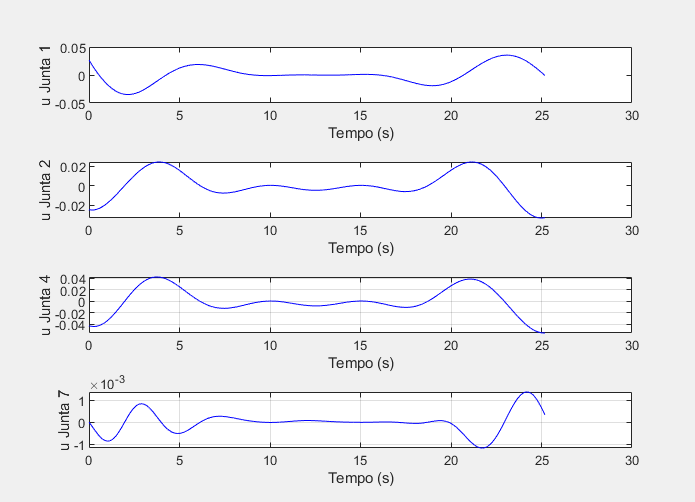
\includegraphics[width=\linewidth]{parte2_u_1.png}
        \caption{Sinais de controle das juntas}
        \label{fig:parte2_u_1}
    \end{subfigure}
    \hfill
    \caption{Gráficos do controle por servo-visão (K = 1)}
    \label{fig:parte2_1}
\end{figure}
É possível notar que o efetuador consegue seguir a trajetória de referência.
Além disso, o gráfico de erro consegue mostrar que o sistema é exponencialmente estável.
Entretanto, para o ganho do controlador sendo K = 1, ainda tem um grande margem de aumento desse ganho para ficar mais próximos dos limites de $|u_i| \leq 1 (i=1,2,4,7)$.
Então, foi feito a sintonização do ganho do controlador satisfazendo a expressão anterior, obtendo K = 37.25 e tendo os seguintes gráficos:
\newpage

\begin{figure}[h!]
    \centering
    \begin{subfigure}[b]{0.27\textwidth}
        \centering
        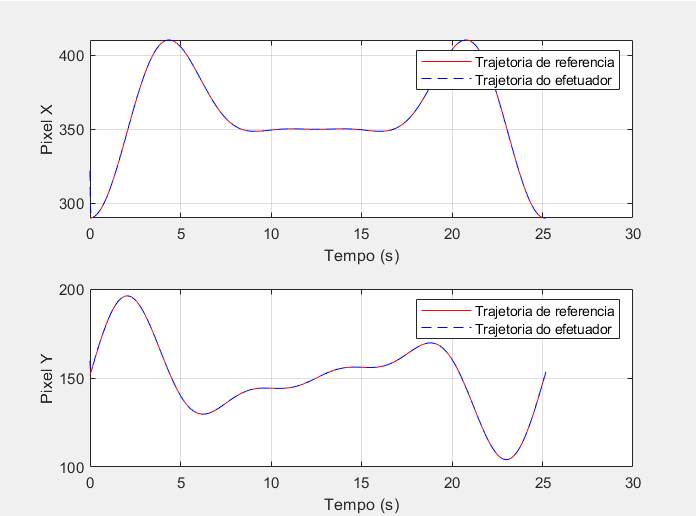
\includegraphics[width=\linewidth]{parte2_trajetorias_2.png}
        \caption{Trajetórias nos eixos X e Y}
        \label{fig:parte2_trajetorias_2}
    \end{subfigure}%
    \hfill
    \begin{subfigure}[b]{0.27\textwidth}
        \centering
        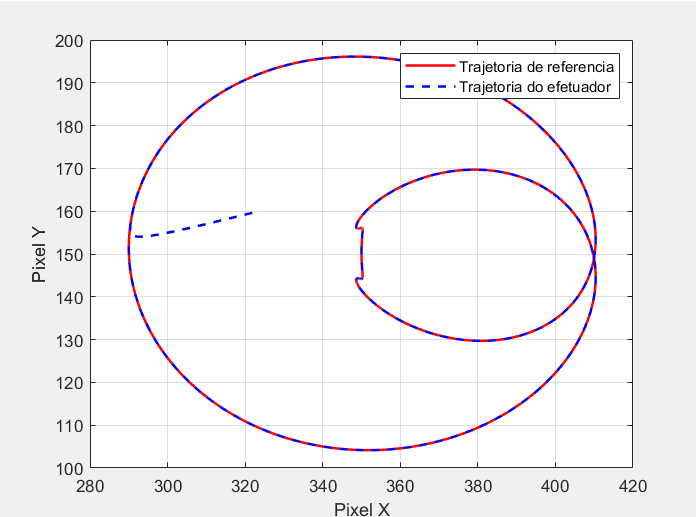
\includegraphics[width=\linewidth]{parte2_trajetoriaxy_2.png}
        \caption{Trajetória no plano X-Y}
        \label{fig:parte2_trajetoriaxy_2}
    \end{subfigure}%
    \hfill
    \begin{subfigure}[b]{0.27\textwidth}
        \centering
        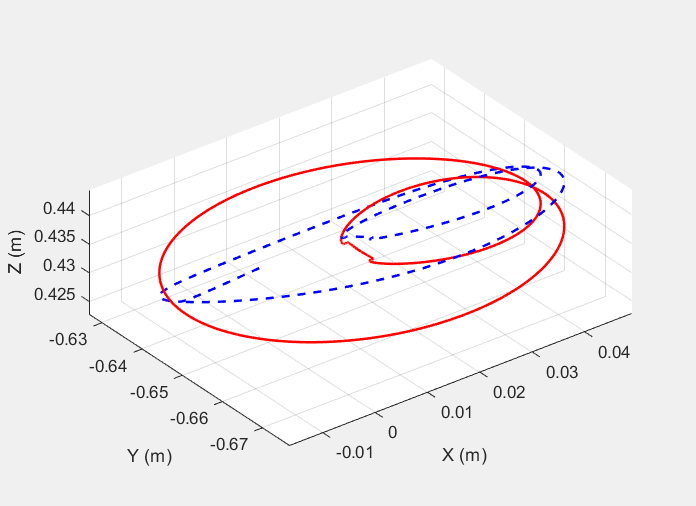
\includegraphics[width=\linewidth]{parte2_trajetoriaxyz_2.png}
        \caption{Trajetória no espaço XYZ}
        \label{fig:parte2_trajetoriaxyz_2}
    \end{subfigure}
    \begin{subfigure}[b]{0.27\textwidth}
        \centering
        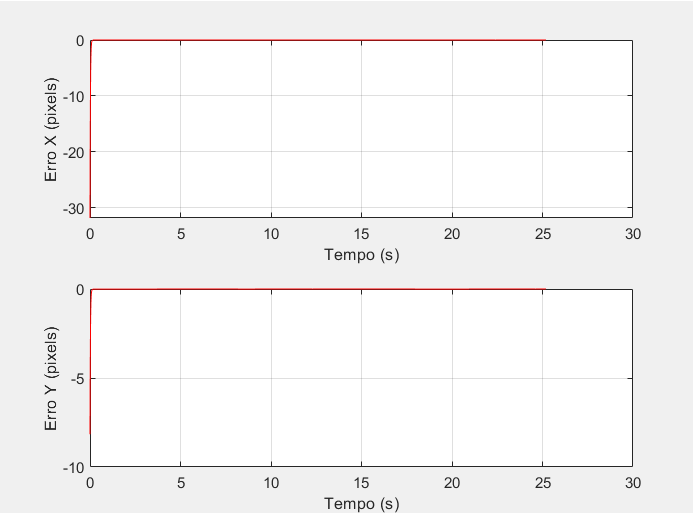
\includegraphics[width=\linewidth]{parte2_erro_2.png}
        \caption{Erro de posição nos eixos X e Y}
        \label{fig:parte2_erro_2}
    \end{subfigure}
    \hspace{2cm}
    \begin{subfigure}[b]{0.27\textwidth}
        \centering
        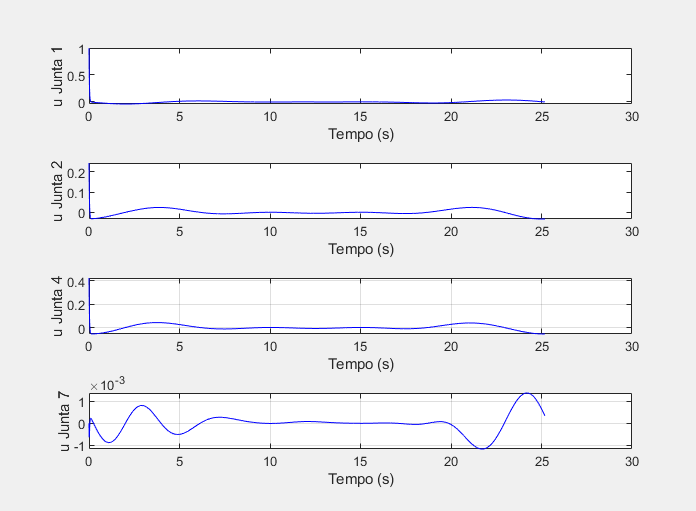
\includegraphics[width=\linewidth]{parte2_u_2.png}
        \caption{Sinais de controle das juntas}
        \label{fig:parte2_u_2}
    \end{subfigure}
    \hfill
    \caption{Gráficos do controle por servo-visão (K = 37.25)}
    \label{fig:parte2_2}
\end{figure}

É possível notar que o erro vai muito mais rápido para zero,
mas possui um sinal de controle das juntas muito maior no começo do seguimento da trajetória.
Além disso, foi feita outra verificação de desempenho do controlador projetado se a câmera é rotacionada em $\phi = \pi/3$
mas esta rotação não é considerada na lei de controle u, i.e. em u tem-se $K_p(\phi = 0)$. Foi obtido o seguinte resultado:

\begin{figure}[h!]
    \centering
    \begin{subfigure}[b]{0.27\textwidth}
        \centering
        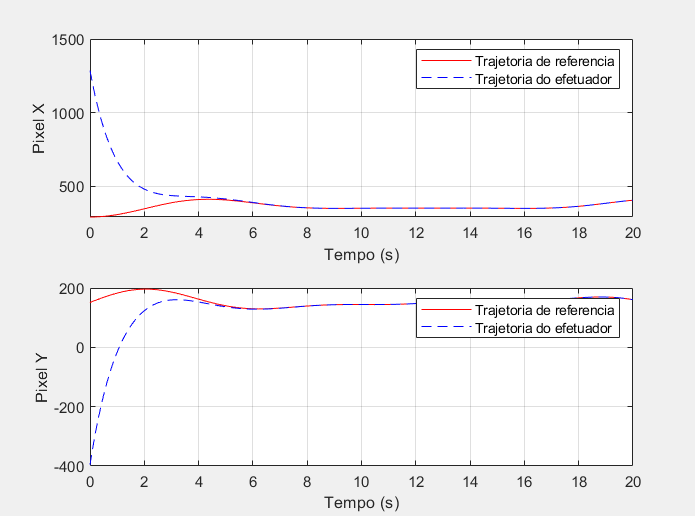
\includegraphics[width=\linewidth]{parte2_trajetorias_3.png}
        \caption{Trajetórias nos eixos X e Y}
        \label{fig:parte2_trajetorias_3}
    \end{subfigure}%
    \hfill
    \begin{subfigure}[b]{0.27\textwidth}
        \centering
        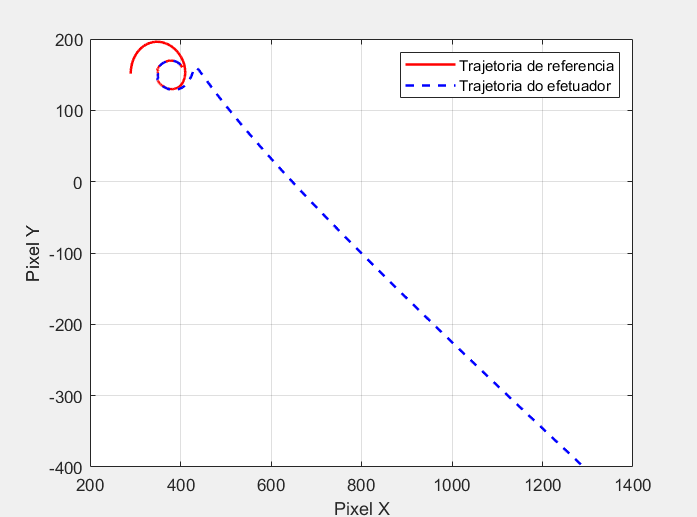
\includegraphics[width=\linewidth]{parte2_trajetoriaxy_3.png}
        \caption{Trajetória no plano X-Y}
        \label{fig:parte2_trajetoriaxy_3}
    \end{subfigure}%
    \hfill
    \begin{subfigure}[b]{0.27\textwidth}
        \centering
        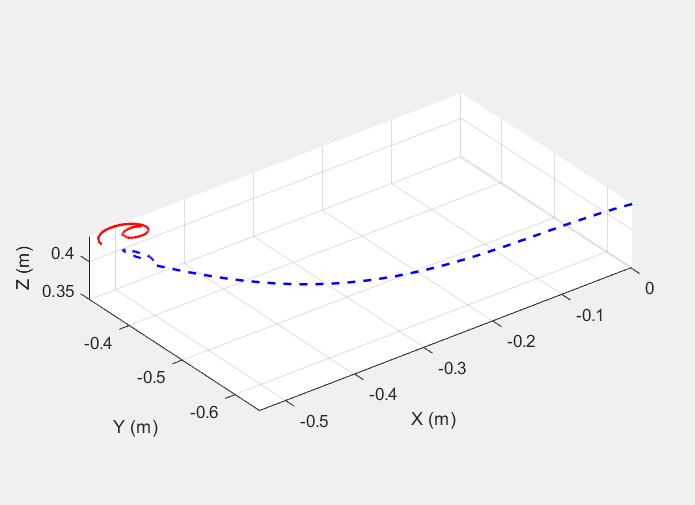
\includegraphics[width=\linewidth]{parte2_trajetoriaxyz_3.png}
        \caption{Trajetória no espaço XYZ}
        \label{fig:parte2_trajetoriaxyz_3}
    \end{subfigure}
    \begin{subfigure}[b]{0.27\textwidth}
        \centering
        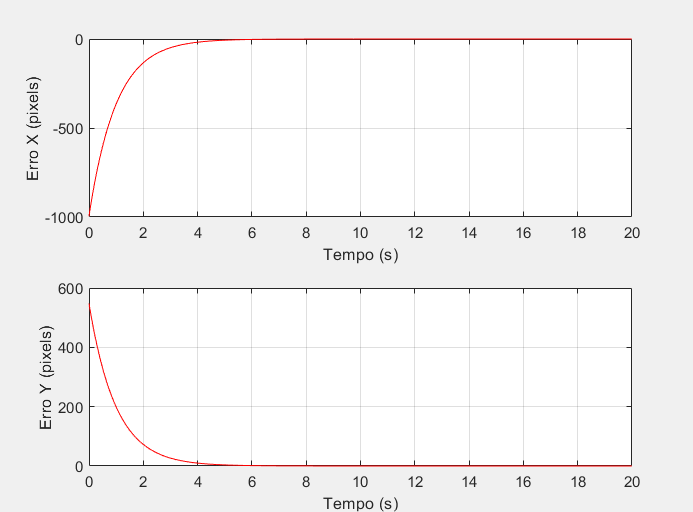
\includegraphics[width=\linewidth]{parte2_erro_3.png}
        \caption{Erro de posição nos eixos X e Y}
        \label{fig:parte2_erro_3}
    \end{subfigure}
    \hspace{2cm}
    \begin{subfigure}[b]{0.27\textwidth}
        \centering
        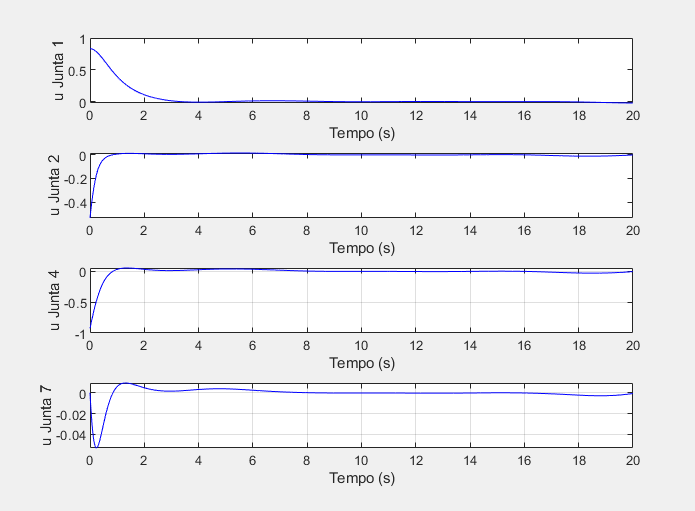
\includegraphics[width=\linewidth]{parte2_u_3.png}
        \caption{Sinais de controle das juntas}
        \label{fig:parte2_u_3}
    \end{subfigure}
    \hfill
    \caption{Gráficos do controle por servo-visão (K = 1, $\phi = \pi/3$ e $K_p(\phi = 0)$)}
    \label{fig:parte2_3}
\end{figure}

Ao analisar os gráficos de trajetórios nos eixos X e Y ao longo tempo e do erro posição nos eixos X e Y dá uma falsa impressão de que o controle funcionou da forma correta.
Porém, fica claro pelos outros gráficos que a trajetória do efetuador divergiu da trajetória da referência.
Porque uma mudança na orientação da câmera sem alterar o controle acaba gerando uma total não conformidade com controle.
Sendo que deveria ter o seguinte comportamento ao alterar a lei de controle para $\phi = \pi/3$.

\begin{figure}[h!]
    \centering
    \begin{subfigure}[b]{0.27\textwidth}
        \centering
        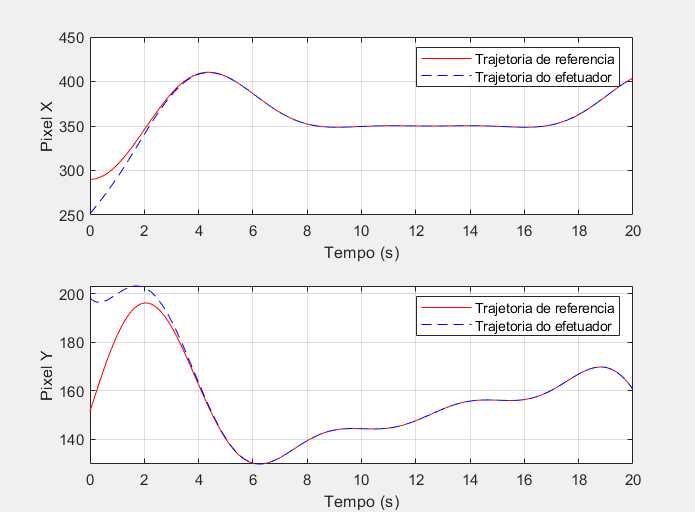
\includegraphics[width=\linewidth]{parte2_trajetorias_4.png}
        \caption{Trajetórias nos eixos X e Y}
        \label{fig:parte2_trajetorias_4}
    \end{subfigure}%
    \hfill
    \begin{subfigure}[b]{0.27\textwidth}
        \centering
        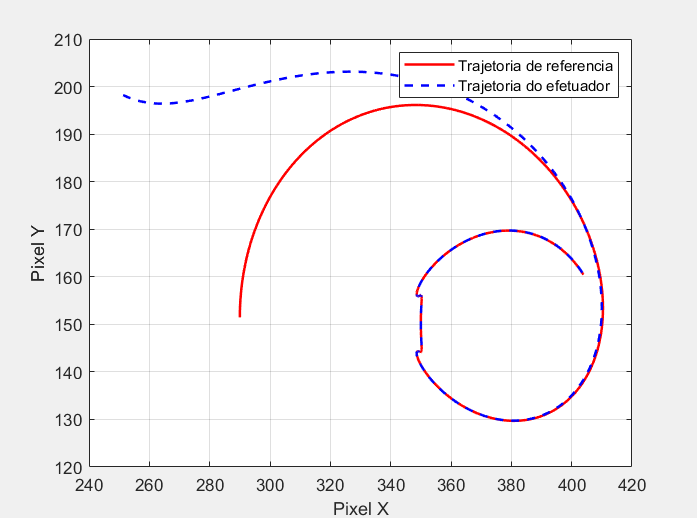
\includegraphics[width=\linewidth]{parte2_trajetoriaxy_4.png}
        \caption{Trajetória no plano X-Y}
        \label{fig:parte2_trajetoriaxy_4}
    \end{subfigure}%
    \hfill
    \begin{subfigure}[b]{0.27\textwidth}
        \centering
        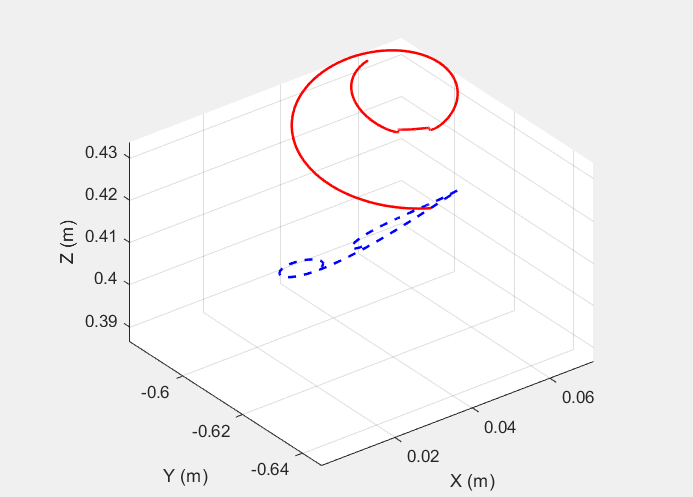
\includegraphics[width=\linewidth]{parte2_trajetoriaxyz_4.png}
        \caption{Trajetória no espaço XYZ}
        \label{fig:parte2_trajetoriaxyz_4}
    \end{subfigure}
    \begin{subfigure}[b]{0.27\textwidth}
        \centering
        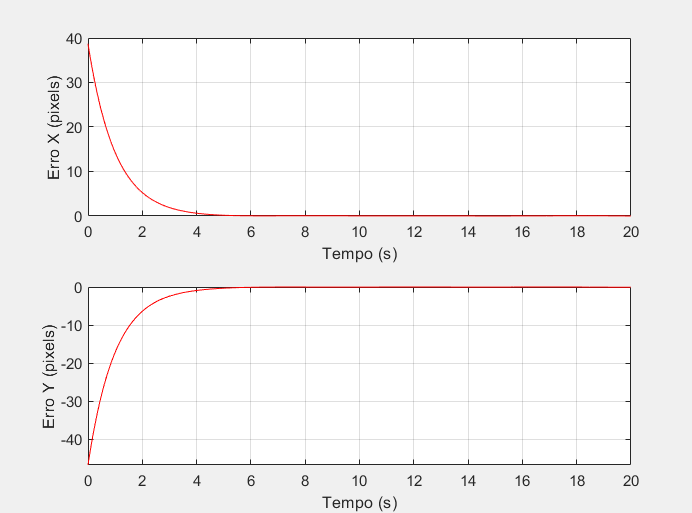
\includegraphics[width=\linewidth]{parte2_erro_4.png}
        \caption{Erro de posição nos eixos X e Y}
        \label{fig:parte2_erro_4}
    \end{subfigure}
    \hspace{2cm}
    \begin{subfigure}[b]{0.27\textwidth}
        \centering
        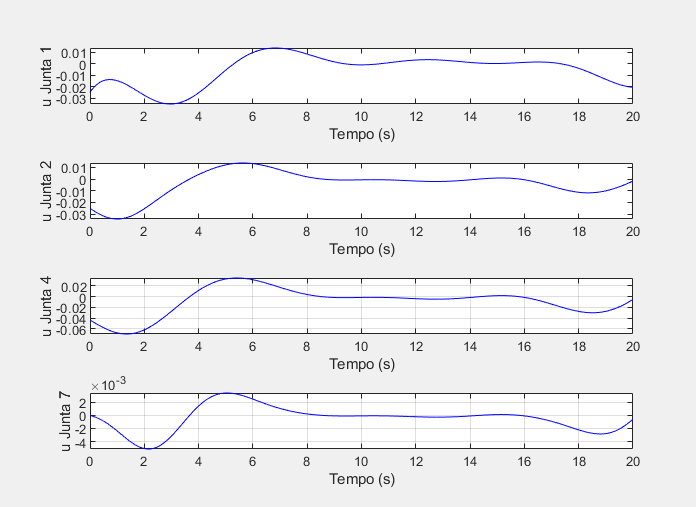
\includegraphics[width=\linewidth]{parte2_u_4.png}
        \caption{Sinais de controle das juntas}
        \label{fig:parte2_u_4}
    \end{subfigure}
    \hfill
    \caption{Gráficos do controle por servo-visão (K = 1, $\phi = \pi/3$ e $K_p(\phi = \pi/3)$)}
    \label{fig:parte2_4}
\end{figure}

\section{Conclusão}

Em resumo, os dois problemas abordados envolvem o controle cinemático de manipuladores com diferentes abordagens.
No primeiro caso, foi possível simular o manipulador Kinova Gen3 e avaliar o desempenho dos controladores, destacando a importância da sintonia dos ganhos para garantir estabilidade e precisão nas trajetórias.
No segundo caso, o controle por servo-visão foi ajustado para garantir que o manipulador seguisse a trajetória desejada, considerando as limitações da câmera e a rotação não considerada na lei de controle.
Ambos os casos ressaltam a importância do planejamento e da sintonia dos controladores para um desempenho estável e preciso.

\newpage

\section*{Apêndice}

\begin{lstlisting}[caption={Código da primeira parte do trabalho}, label={code:subsecao21}]
clear all;

% Definicao dos parametros DH com juntas revolutas
L(1) = Revolute('d', -0.2848, 'a', 0, 'alpha', pi/2, 'offset', 0);
L(2) = Revolute('d', -0.0118, 'a', 0, 'alpha', pi/2, 'offset', pi);
L(3) = Revolute('d', -0.4208, 'a', 0, 'alpha', pi/2, 'offset', pi);
L(4) = Revolute('d', -0.0128, 'a', 0, 'alpha', pi/2, 'offset', pi);
L(5) = Revolute('d', -0.3143, 'a', 0, 'alpha', pi/2, 'offset', pi);
L(6) = Revolute('d', 0,       'a', 0, 'alpha', pi/2, 'offset', pi);
L(7) = Revolute('d', 0,       'a', 0, 'alpha', pi,   'offset', pi);

% Criacao do manipulador
kinova = SerialLink(L, 'name', 'Kinova');
kinova.base = trotx(180);  % Define a base do robo

% Condicoes iniciais
q0 = deg2rad([0, 15, 180, -130, 0, 55, 90]);

% Inicializacao de variaveis
qi = q0;
h = 0.01; % Passo de tempo
tmax = 20; % Tempo maximo (s)
wmax = 1; % Velocidade maxima das juntas (rad/s)
wn = pi/2; % Frequencia natural
wn3 = pi/8; % Frequencia natural - Terceira Trajetoria

K = 1.81; % Ganho do controlador 1 da trajetoria (a)
% K = 2.05; % Ganho do controlador 1 da trajetoria (b)
% K = 1.99; % Ganho do controlador 1 da trajetoria (c)
% K = 1.39; % Ganho do controlador 2 da trajetoria (a)
% K = 2.42; % Ganho do controlador 2 da trajetoria (b)
% K = 1.10; % Ganho do controlador 2 da trajetoria (c)

% Vetores para armazenamento dos dados
t_vec = 0:h:tmax;
x_ref = zeros(3, length(t_vec));
x_out = zeros(3, length(t_vec));
u_vec = zeros(4, length(t_vec)); % Para armazenar os 4 primeiros valores de u

% Simulacao
for k = 1:length(t_vec)
    t = t_vec(k);
    
    % Jacobiano e cinematica direta
    J = kinova.jacob0(qi); % Jacobiano do robo
    Jp = J(1:3,1:7);
    x = kinova.fkine(qi).t; % Posicao atual do fim do braco
    
    % Selecionar a trajetoria desejada:
    xdd=0;
    
    % Trajetoria (a)
    xd = routeGen1(t, wn);
    % xdd = routeGen1Deriv(t, wn);
    
    % Trajetoria (b)
    % xd = routeGen2(t, wn);
    % xdd = routeGen2Deriv(t, wn);
    
    % Trajetoria (c)
    % xd = routeGen3(t, wn3);
    % xdd = routeGen3Deriv(t, wn3);
    
    % Erro de posicao e velocidade desejada
    err = xd - x; % Erro de posicao
    
    % Controlador
    u = pinv(Jp) * (xdd + K * err); % Calculo das velocidades para as primeiras 4 juntas
    
    % Verificar se algum valor de u e maior que 1
    if any(abs(u) > 1)
        disp('Alerta: Um ou mais valores de u excedem 1.');
        disp('Valores de u:');
        disp(u);
    end
    
    % Integracao (Euler) para as primeiras 4 juntas
    qk = qi; % Copia o vetor atual de juntas
    qk = qi + h * u'; % Atualiza apenas as primeiras 4 juntas
    qi = qk; % Atualiza o estado
    
    % Armazenar dados
    x_ref(:, k) = xd; % Trajetoria de referencia
    x_out(:, k) = x;  % Trajetoria saida
    u_vec(:, k) = u(1:4); % Armazena os 4 primeiros valores de u
end

% Plotagem dos resultados
figure;
subplot(3, 1, 1);
plot(t_vec, x_ref(1, :), 'r', 'LineWidth', 1.5); hold on;
plot(t_vec, x_out(1, :), 'b--', 'LineWidth', 1.5);
xlabel('Tempo (s)');
ylabel('Posicao X (m)');
legend('Referencia', 'Saida');
grid on;

subplot(3, 1, 2);
plot(t_vec, x_ref(2, :), 'r', 'LineWidth', 1.5); hold on;
plot(t_vec, x_out(2, :), 'b--', 'LineWidth', 1.5);
xlabel('Tempo (s)');
ylabel('Posicao Y (m)');
legend('Referencia', 'Saida');
grid on;

subplot(3, 1, 3);
plot(t_vec, x_ref(3, :), 'r', 'LineWidth', 1.5); hold on;
plot(t_vec, x_out(3, :), 'b--', 'LineWidth', 1.5);
xlabel('Tempo (s)');
ylabel('Posicao Z (m)');
legend('Referencia', 'Saida');
grid on;

% Grafico 3D da trajetoria real e desejada
figure;
plot3(x_ref(1, :), x_ref(2, :), x_ref(3, :), 'r-', 'LineWidth', 1.5); hold on;
plot3(x_out(1, :), x_out(2, :), x_out(3, :), 'b--', 'LineWidth', 1.5);
xlabel('X (m)');
ylabel('Y (m)');
zlabel('Z (m)');
legend('Referencia', 'Saida');
grid on;

% Graficos das velocidades das 4 primeiras juntas
figure;

subplot(4, 1, 1);
plot(t_vec, u_vec(1, :), 'r', 'LineWidth', 1.5);
xlabel('Tempo (s)');
ylabel('u_1 (rad/s)');
grid on;

subplot(4, 1, 2);
plot(t_vec, u_vec(2, :), 'b', 'LineWidth', 1.5);
xlabel('Tempo (s)');
ylabel('u_2 (rad/s)');
grid on;

subplot(4, 1, 3);
plot(t_vec, u_vec(3, :), 'g', 'LineWidth', 1.5);
xlabel('Tempo (s)');
ylabel('u_3 (rad/s)');
grid on;

subplot(4, 1, 4);
plot(t_vec, u_vec(4, :), 'm', 'LineWidth', 1.5);
xlabel('Tempo (s)');
ylabel('u_4 (rad/s)');
grid on;

% Calculo do erro ao longo do tempo
error_x = x_ref(1, :) - x_out(1, :); % Erro no eixo X
error_y = x_ref(2, :) - x_out(2, :); % Erro no eixo Y
error_z = x_ref(3, :) - x_out(3, :); % Erro no eixo Z

% Graficos do erro em subplots
figure;

subplot(3, 1, 1);
plot(t_vec, error_x, 'r', 'LineWidth', 1.5);
xlabel('Tempo (s)');
ylabel('Erro X (m)');
grid on;

subplot(3, 1, 2);
plot(t_vec, error_y, 'g', 'LineWidth', 1.5);
xlabel('Tempo (s)');
ylabel('Erro Y (m)');
grid on;

subplot(3, 1, 3);
plot(t_vec, error_z, 'b', 'LineWidth', 1.5);
xlabel('Tempo (s)');
ylabel('Erro Z (m)');
grid on;

% Funcoes de geracao de trajetoria
function xd = routeGen1(t, wn)
    % Trajetoria (a): Circunferencia no plano X-Z
    r = 0.1; % Raio da circunferencia
    x0 = [0.4; 0; 0.4]; % Centro da circunferencia
    xd = x0 + [r * cos(wn * t); 0; r * sin(wn * t)];
end

function xdot = routeGen1Deriv(t, wn)
    % Derivada da trajetoria (a): Velocidade da circunferencia no plano X-Z
    r = 0.1; % Raio da circunferencia
    xdot = [-r * wn * sin(wn * t); 0; r * wn * cos(wn * t)];
end

function xd = routeGen2(t, wn)
    % Trajetoria (b): Espiral no plano X-Z
    r = 0.1; % Raio inicial
    x0 = [0.4; 0; 0.4]; % Centro da espiral
    xd = x0 + [r * cos(wn * t); 0; r * sin(wn * t)];
end

function xdot = routeGen2Deriv(t, wn)
    % Derivada da trajetoria (b): Velocidade da espiral no plano X-Z
    r = 0.1; % Raio inicial
    xdot = [-r * wn * sin(wn * t); 0; r * wn * cos(wn * t)];
end

function xd = routeGen3(t, wn)
    % Trajetoria (c): Linha reta no eixo X
    x0 = [0.4; 0; 0.4]; % Ponto inicial
    xf = [0.5; 0; 0.5]; % Ponto final
    xd = x0 + (xf - x0) * sin(wn * t);
end

function xdot = routeGen3Deriv(t, wn)
    % Derivada da trajetoria (c): Velocidade da linha reta no eixo X
    x0 = [0.4; 0; 0.4]; % Ponto inicial
    xf = [0.5; 0; 0.5]; % Ponto final
    xdot = (xf - x0) * cos(wn * t) * wn;
end      
\end{lstlisting}

\newpage

\begin{lstlisting}[caption={Código da segunda parte do trabalho}, label={code:subsecao22}]
clear all; close all;

% Definicao dos parametros DH com juntas revolutas
L(1) = Revolute('d', -0.2848, 'a', 0, 'alpha', pi/2, 'offset', 0); % Parametro da junta 1
L(2) = Revolute('d', -0.0118, 'a', 0, 'alpha', pi/2, 'offset', pi); % Parametro da junta 2
L(3) = Revolute('d', -0.4208, 'a', 0, 'alpha', pi/2, 'offset', pi); % Parametro da junta 3
L(4) = Revolute('d', -0.0128, 'a', 0, 'alpha', pi/2, 'offset', pi); % Parametro da junta 4
L(5) = Revolute('d', -0.3143, 'a', 0, 'alpha', pi/2, 'offset', pi); % Parametro da junta 5
L(6) = Revolute('d', 0,       'a', 0, 'alpha', pi/2, 'offset', pi); % Parametro da junta 6
L(7) = Revolute('d', -0.3574, 'a', 0, 'alpha', pi,   'offset', pi); % Parametro da junta 7

% Criacao do manipulador
kinova_gen3 = SerialLink(L, 'name', 'Kinova'); % Criacao do modelo do manipulador
kinova_gen3.base = trotx(180);  % Define a base do robo (rotacao em torno do eixo X)

% Parametros do sistema
f = 4e-3; % Distancia focal da camera (m)
z0 = 0.4338; % Profundidade inicial (m)
alpha = 200000; % Fator de escala (pixels/m)
Oc = [320; 240]; % Origem do plano da imagem (pixels)
Pbc = [0;-0.603; 0]; % Posicao da camera em relacao a base (m)
phi = 0; % Angulo de orientacao da camera (rad)
phi_trocado = pi/3; % Angulo de orientacao da camera trocado (rad)
wn = 0.5; % Frequencia angular (rad/s)

% Ganho do controlador
K = 1; % Ajuste o ganho conforme necessario para o controlador

% Trajetoria desejada no plano da imagem
h = 0.01; % Passo de tempo
tmax = 20; % Tempo maximo (s)
t = 0:h:tmax; % Vetor de tempo para simulacao
xcd = [
    360- 30*cos(wn*t)- 30*cos(1.5*wn*t)- 10*cos(2*wn*t); % Trajetoria no eixo X
    150- 20*cos(wn*t + 1.6)- 20*cos(1.5*wn*t + 1.6)- 10*cos(2*wn*t + 1.6) % Trajetoria no eixo Y
];
xcdd = [
    30*sin(wn*t)*wn + 30*sin(1.5*wn*t)*1.5*wn + 10*sin(2*wn*t)*2*wn; % Derivada da trajetoria no eixo X
    20*sin(wn*t + 1.6)*wn + 20*sin(1.5*wn*t + 1.6)*1.5*wn + 10*sin(2*wn*t + 1.6)*2*wn % Derivada da trajetoria no eixo Y
];

% Transformacao camera/espaco de trabalho
Kp = (f / z0) * diag([alpha,-alpha]) * [cos(phi), sin(phi); sin(phi),-cos(phi)]; 
% Kp = (f / z0) * diag([alpha,-alpha]) * [cos(phi_trocado), sin(phi_trocado); sin(phi_trocado),-cos(phi_trocado)];
% Matriz de projecao da camera no plano da imagem
xc0 = (f / z0) * diag([alpha,-alpha]) * [-cos(phi),-sin(phi);-sin(phi), cos(phi)]*Pbc(1:2) + Oc;
% xc0 = (f / z0) * diag([alpha,-alpha]) * [-cos(phi_trocado),-sin(phi_trocado);-sin(phi_trocado), cos(phi_trocado)]*Pbc(1:2) + Oc;
% Posiçao inicial da camera no plano da imagem

% Inicializacao de variaveis
xc = zeros(2, length(t)-1); % Posicao no plano da imagem
theta = deg2rad([90; 15; 180;-130; 0; 55; 0]); % Angulos iniciais das juntas (rad)
theta_log = zeros(length(theta), length(t)-1); % Log para salvar os valores de theta
xyz = zeros(3, length(t)-1); % Posicao no espaco do efetuador (x, y, z)

% Erros
ex = zeros(1, length(t)-1); % Erro no eixo X
ey = zeros(1, length(t)-1); % Erro no eixo Y
u_log = zeros(4, length(t)-1); % Log para salvar os valores de u

% Simulacao do movimento
for k = 1:length(t)-1
    % Cinematica direta (posicao no espaco de trabalho)
    x = kinova_gen3.fkine(theta).t; % Calcula a posicao do efetuador
    xyz(:, k) = x; % Salva a posicao do efetuador no espaco (x, y, z)
    
    % Projecao no plano da imagem
    xc(:, k) = Kp * x(1:2) + xc0; % Calcula a posicao projetada no plano da imagem
    
    % Erro na imagem (diferenca entre a trajetoria desejada e a atual)
    ecd = xcd(:, k)- xc(:, k);
    ex(k) = ecd(1); % Erro no eixo X
    ey(k) = ecd(2); % Erro no eixo Y
    
    % Jacobiano do manipulador (somente juntas controladas)
    J = kinova_gen3.jacob0(theta); % Jacobiano completo
    J_reduced = J(1:2, [1, 2, 4, 6]); % Considera apenas as colunas das juntas 1, 2, 4 e 6
    
    % Controle cinemático
    Jv = Kp * J_reduced; % Controle baseado no Jacobiano reduzido
    xcd_dot = xcdd(:, k); % Derivada da trajetoria desejada
    u = pinv(Jv) * (xcd_dot + K * ecd); % Calcula o comando de controle
    
    % Verificar se algum valor de u é maior que 1
    if any(abs(u) > 1)
        disp('Alerta: Um ou mais valores de u excedem 1.');
        disp('Valores de u:');
        disp(u);
    end
    
    % Atualizacao dos angulos das juntas
    theta_log(:, k) = theta; % Salva os angulos das juntas
    theta([1, 2, 4, 6]) = theta([1, 2, 4, 6]) + u * h; % Atualiza os angulos com o controle
    
    % Log de u
    u_log(:, k) = u;
end

% Graficos para visualizacao dos resultados
figure;
subplot(2, 1, 1);
plot(t(1:end-1), xcd(1, 1:end-1), 'r', t(1:end-1), xc(1, :), 'b--');
xlabel('Tempo (s)'); ylabel('Pixel X');
legend('Trajetoria de referencia', 'Trajetoria do efetuador');
grid on;

subplot(2, 1, 2);
plot(t(1:end-1), xcd(2, 1:end-1), 'r', t(1:end-1), xc(2, :), 'b--');
xlabel('Tempo (s)'); ylabel('Pixel Y');
legend('Trajetoria de referencia', 'Trajetoria do efetuador');
grid on;

figure; % Grafico XY (trajetoria no plano da tela)
plot(xcd(1, :), xcd(2, :), 'r', 'LineWidth', 1.5); hold on;
plot(xc(1, :), xc(2, :), 'b--', 'LineWidth', 1.5);
xlabel('Pixel X'); ylabel('Pixel Y');
legend('Trajetoria de referencia', 'Trajetoria do efetuador');
grid on;

% Grafico XYZ (trajetoria no espaco do efetuador)
xdr = pinv(Kp)*(xcd-xc0);
zdr = z0*ones(size(xcd(1,:)));
figure;
plot3(xdr(1, :), xdr(2, :), zdr, 'r-', 'LineWidth', 1.5); hold on;
plot3(xyz(1, :), xyz(2, :), xyz(3, :), 'b--', 'LineWidth', 1.5);
xlabel('X (m)'); ylabel('Y (m)'); zlabel('Z (m)');
grid on; axis equal;

% Grafico de erro
figure;
subplot(2, 1, 1);
plot(t(1:end-1), ex, 'r', 'LineWidth', 1.5);
xlabel('Tempo (s)'); ylabel('Erro no X');
grid on;

subplot(2, 1, 2);
plot(t(1:end-1), ey, 'r', 'LineWidth', 1.5);
xlabel('Tempo (s)'); ylabel('Erro no Y');
grid on;
\end{lstlisting}

\end{document}